% !TeX root = main.tex


%% newCommand
% voltages
\newcommand{\Ua}{U_{\mathrm{a}}}
\newcommand{\Ui}{U_{\mathrm{i}}}
\newcommand{\Uan}{U_{\mathrm{a,n}}}


% current
\newcommand{\Ia}{I_{\mathrm{a}}}
\newcommand{\In}{I_{\mathrm{n}}}

% resistor
\newcommand{\Ra}{R_{\mathrm{a}}}

% power
\newcommand{\Pn}{P_{\mathrm{n}}}
\newcommand{\Pl}{P_{\mathrm{l}}}
\newcommand{\Pfe}{P_{\mathrm{Fe}}}
\newcommand{\Pcu}{P_{\mathrm{Cu,a}}}

% torque
\newcommand{\Tn}{T_{\mathrm{n}}}

% speed
\newcommand{\nN}{n_{\mathrm{n}}}
\newcommand{\nO}{n_{\mathrm{0}}}

% flux
\newcommand{\phiDelta}{\phi_{\updelta}}

% machine design related parameter
\newcommand{\za}{z_{\mathrm{a}}}
\newcommand{\taup}{\tau_{\mathrm{p}}}
\newcommand{\lz}{l_{\mathrm{z}}}




%% add [solution]
\documentclass[solution]{exerciseClass}

%%%%%%%%%%%%%%%%%%%%%%%%%%%%%%%%%%%%%%%%%%%%%%%%%%%%%%%%%%%%%%%%%%%%%%%%%%%%%
%%%Lecture Include Only%%%
\includeonly{tex/exercise03}
%%%%%%%%%%%%%%%%%%%%%%%%%%%%%%%%%%%%%%%%%%%%%%%%%%%%%%%%%%%%%%%%%%%%%%%%%%%%%

\begin{document}

    %%%%%%%%%%%%%%%%%%%%%%%%%%%%%%%%%%%%%%%%%%%%%%%%%%%%%%%%%%%%%
%% Begin exercise %%
%%%%%%%%%%%%%%%%%%%%%%%%%%%%%%%%%%%%%%%%%%%%%%%%%%%%%%%%%%%%%
\ex{Fundamentals of the magnetic field}


\normalsize{\textbf{Acknowledgement}: The following exercise is adapted from ``Elektrische Maschinen und Antriebe Übungsbuch: Aufgapen mit Lösungsweg'' by A. Binder, Springer, 2017}\\



%%%%%%%%%%%%%%%%%%%%%%%%%%%%%%%%%%%%%%%%%%%%%%%%%%%%%%%%%%%%%
%% Task 1 %%
%%%%%%%%%%%%%%%%%%%%%%%%%%%%%%%%%%%%%%%%%%%%%%%%%%%%%%%%%%%%%

\task{Magnetic iron yoke}
The iron core consists of thin single metal sheets with a cross-sectional area of $A$ = 900 $\si{mm}^2$ and with an air gap of $\delta$ = 3 mm. A simplified sketch is shown in Fig.~\ref{fig:MagneticIronCircle}. The material behavior of the selected iron is visualized in Fig.~\ref{fig:BH_curve}. The coil with $N$ turns contains a direct current which results in a homogeneous magnetic flux density of $B_{\mathrm{\delta}}$ = 1.8 T in the air gap.


\begin{figure}[htb]
    \centering
    \import{./fig/ex01/}{MagneticIronCircle.pdf_tex}
    \caption{Simplified sketch of a magnetic iron core. All dimensions of the core are given in mm.}
    \label{fig:MagneticIronCircle}
\end{figure}

\begin{figure}[htb]
    \centering
    \import{./fig/ex01/}{BH_curve.pdf_tex}
    \caption{Direct current magnetization curves of electrical steel for (1) hot rolled processing with a thickness of 0.5 mm and (2) cold rolled processing with a thickness of 0.35 mm. The magnetization curve in figure on the left side is a zoomed version of material (1) for lower field strengths.}
    \label{fig:BH_curve}
\end{figure}


%%%%%%%%%%%%%%%%%%%%%%%%%%%%%%%%%%%%%%%%%%%%%%%%%%%%%%%%%%%%%

\subtask{Calculate the magnetic flux $\phi_{\mathrm{\updelta}}$ in the air gap.}
\begin{solutionblock}
    The area of the air gap is equal to the iron core area ($A_{\mathrm{\updelta}} = A = 900 \ \si{mm^2}$).
    The calculation of the magnetic flux is defined as follows:
    \begin{equation}
        \phi_{\updelta} = \int_{S}^{} \boldsymbol{B} \ \mathrm{d} \boldsymbol{S}
        = B A,
    \end{equation}
    where $\boldsymbol{B}$ is the magnetic flux density and $\boldsymbol{S}$ is the surface area to integrate. The above integral could be simplified to B*A because the flux density is homogeneous and the integration surface S  and the flux are perpendicular to each other. 
    This results in
    \begin{equation}
        \phi_{\updelta}  = B_{\updelta} A_{\updelta}
        = 1.8 \ \si{T} \cdot 900 \cdot 10^{-6} \ \si{m^2}
        = 1.62 \ \mathrm{mWb}.
    \end{equation}

\end{solutionblock}



%%%%%%%%%%%%%%%%%%%%%%%%%%%%%%%%%%%%%%%%%%%%%%%%%%%%%%%%%%%%%

\subtask{How big is the magnetic flux density $B_{\mathrm{Fe}}$ in the iron core at the dotted line in Fig.~\ref{fig:MagneticIronCircle}? Neglect the leakage flux.}
\begin{solutionblock}
    Since the leakage flux is neglected, the fluxes $\phi_{\mathrm{\updelta}}$ in the air gap and $\phi_{\mathrm{Fe}}$ in the iron are equal. This results in the following equation:
    \begin{equation}
        \phi_{\mathrm{\updelta}} = \phi_{\mathrm{Fe}}
        = A_{\mathrm{\updelta}} B_{\mathrm{\updelta}}
        = A_{\mathrm{Fe}} B_{\mathrm{Fe}}.
    \end{equation}

    The equation from above is resorted to calculate the magnetic flux density:
    \begin{equation}
        B_{\mathrm{Fe}} = B_{\mathrm{\updelta}} \frac{A_{\mathrm{\updelta}}}{A_{\mathrm{Fe}}} = 1.8 \ \si{T}.
    \end{equation}

\end{solutionblock}


%%%%%%%%%%%%%%%%%%%%%%%%%%%%%%%%%%%%%%%%%%%%%%%%%%%%%%%%%%%%%

\subtask{What is the value of the permeability $\mu$ and the magnetic field strengths $H_{\mathrm{\updelta}}$ and $H_{\mathrm{Fe}}$ in the air gap and in the iron for the given operating point?}
\begin{solutionblock}
    The permeability in the air gap is equal to the permeability in the air, which is given with: \newline $\mu = \mu_{\mathrm{0}} = 4 \pi \cdot 10^{-7} \ \frac{\si{Vs}}{\si{Am}}$. The magnetic field strength in the air gap is calculated with:
    \begin{equation}
        H_{\mathrm{\updelta}} = \frac{B_{\mathrm{\updelta}}}{\mu_{\mathrm{0}}}
        = \frac{1.8 \ \si{T}}{4 \pi \cdot 10^{-7} \ \frac{\si{Vs}}{\si{Am}}}
        = 1432395 \ \frac{\si{A}}{\si{m}}.
    \end{equation}

    The curve (1) on the left side in Fig.~\ref{fig:BH_curve} shows for $B_{\mathrm{Fe}}$ = 1.8 \si{T} a magnetic filed strength of \newline $H_{\mathrm{Fe}} = 80 \ \frac{\si{A}}{\si{cm}}$ = $8000 \ \frac{\si{A}}{\si{m}}$. With the filed strength $H_{\mathrm{Fe}}$ the permeability of the iron is calculated:
    \begin{equation}
        \mu_{\mathrm{Fe}} = \frac{B_{\mathrm{Fe}}}{H_{\mathrm{Fe}}}
        = \frac{1.8 \ \si{T}}{8000 \ \si{A/m}}
        = 0.000225 \ \frac{\si{Vs}}{\si{Am}},
    \end{equation}
    which is approximately 179 times $\mu_{\mathrm{0}}$.

\end{solutionblock}



%%%%%%%%%%%%%%%%%%%%%%%%%%%%%%%%%%%%%%%%%%%%%%%%%%%%%%%%%%%%%

\subtask{What is the required electromotive force $\theta = N \cdot I$ in the excitation coil to excite the flux density $B_{\mathrm{\updelta}}$ = 1.8 T?}
\begin{solutionblock}

    The electromotive force is calculated with Ampère's law along closed curve $\partial S$:
    \begin{equation}
        \theta = N I
        = H_{\updelta} \delta + H_{\mathrm{Fe}} l_{\mathrm{Fe}}.
    \end{equation}
    Therefore, the length of the magnetic path calculates as:
    \begin{equation}
        l_{\mathrm{Fe}} = 2(120-30) + 2(135-30)-3 = 387 \ \si{mm}.
    \end{equation}
    Hence, with the two equations from above, the electromotive force is calculated with:
    \begin{align}
        \begin{split}
            \theta &= H_{\updelta} \delta + H_{\mathrm{Fe}} l_{\mathrm{Fe}}.\\
            &= 1432395 \ \si{A/m} \cdot 0.003 \ \si{m} + 8000 \ \si{A/m} \cdot 0.387 \ \si{m} \\
            &= 7393 \ \si{A}.
        \end{split}
    \end{align}

\end{solutionblock}



%%%%%%%%%%%%%%%%%%%%%%%%%%%%%%%%%%%%%%%%%%%%%%%%%%%%%%%%%%%%%

\subtask{What is the required current $I$ if the coil has $N$ = 500 turns?}
\begin{solutionblock}
    The current is calculated with:
    \begin{equation}
        I = \frac{\theta}{N} = \frac{7393 \ \si{A}}{500} = 14.79 \ \si{A}.
    \end{equation}

\end{solutionblock}






%%%%%%%%%%%%%%%%%%%%%%%%%%%%%%%%%%%%%%%%%%%%%%%%%%%%%%%%%%%%%
%% Task 2 %%
%%%%%%%%%%%%%%%%%%%%%%%%%%%%%%%%%%%%%%%%%%%%%%%%%%%%%%%%%%%%%


\task{Electromagnetic induction}
A magnetic circuit (cf. Fig.~\ref{fig:MagneticIron3D}) has the dimension of $\delta$ = 3 mm, $b$ = $l$ = 30 mm. The excitation coil with $N$ = 500 tuns id fed with an alternating current $i(t) = \hat{I} \sin(2\pi f t)$ with $f$ = 100 Hz and $\hat{I}$ = 7.8 A.
The permeability of the iron $\mu_{\mathrm{Fe}}$ is assumed to be infinite and the flux leakage can be neglected.
A quadratic, non-moving coil with a side length of 30 mm and $N_{\mathrm{C}}$ = 10 turns is within the air gap of the yoke. The orientation of the coil is shown in Fig.~\ref{fig:CoilSurface}. 

\begin{figure}[htb]
    \centering
    \begin{subfigure}[b]{0.4\textwidth}
        \centering
        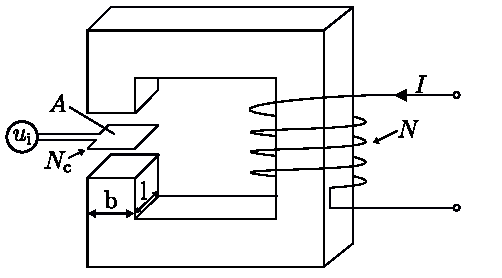
\includegraphics{ex01/MagneticIron3D.pdf}
        \caption{Iron yoke with a coil in the air gap.}
        \label{fig:MagneticIron3D}
    \end{subfigure}
    \quad
    \begin{subfigure}[b]{0.4\textwidth}
        \centering
        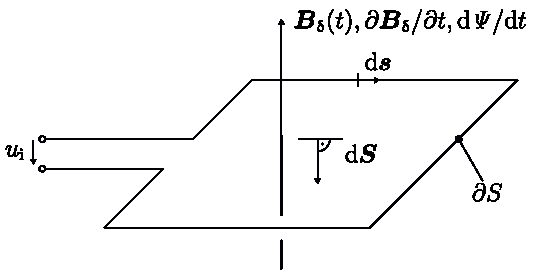
\includegraphics{ex01/CoilSurface.pdf}
        \caption{Orientation of the coil surface in the air gap of the given yoke.}
        \label{fig:CoilSurface}
    \end{subfigure}
    \caption{Iron yoke and coil orientation.}
\end{figure}





%%%%%%%%%%%%%%%%%%%%%%%%%%%%%%%%%%%%%%%%%%%%%%%%%%%%%%%%%%%%%

\subtask{Calculate the flux density $B_{\mathrm{\updelta}}(t)$ in the air gap.
Sketch the trajectories of $i(t)$ and $B_{\mathrm{\updelta}}(t)$.}
\begin{solutionblock}

    Since the leakage flux is neglected, the fluxes $\phi_{\mathrm{\updelta}}$ in the air gap and $\phi_{\mathrm{Fe}}$ in the iron are equal ($\phi_{\mathrm{\updelta}} = \phi_{\mathrm{Fe}}$). In addition, the area of the coil and the air gap area are identical ($A_{\mathrm{Fe}} = A_{\mathrm{\updelta}}$).
    Therefore, the following relationship is made:
    \begin{equation}
        \phi_{\mathrm{\updelta}} = \phi_{\mathrm{Fe}}
        = A_{\mathrm{\updelta}} B_{\mathrm{\updelta}}
        = A_{\mathrm{Fe}} B_{\mathrm{Fe}}.
    \end{equation}
    By resorting the equation from above, the flux density in the air gap is calculated:
    \begin{equation}
        B_{\mathrm{Fe}} = B_{\mathrm{\updelta}} \frac{A_{\mathrm{\updelta}}}{A_{\mathrm{Fe}}} = B_{\mathrm{\updelta}}.
    \end{equation}
    
    The magnetic field strength calculates as:
    \begin{equation}
        H_{\mathrm{Fe}} = \frac{B_{\mathrm{Fe}}}{\mu_{\mathrm{Fe}}} = 0,
    \end{equation}
    which is zero due to the assumption of an infinite permeability in the iron path.

    In the following equation, Ampère's law is given with:
    \begin{equation}
        \theta(t) = N i(t)
        = H_{\mathrm{\updelta}} \delta + H_{\mathrm{Fe}} l_{\mathrm{Fe}}.
    \end{equation}
        
    This equation simplifies by neglecting the magnetic field strength within the iron ($H_{\mathrm{Fe}}$ = 0) due to the infinite permeability. This leads to the following equation:
    \begin{equation}
        \theta(t) = H_{\mathrm{\updelta}} \delta
        = \frac{B_{\mathrm{\updelta}} \delta}{\mu_{\mathrm{0}}},
    \end{equation}
    where $H_{\updelta}$ = $B_{\updelta} \ / \ \mu_{\mathrm{0}}$.

    By rearranging the equation from above, the magnetic flux density in the air gap is calculated as follows:
    \begin{equation}
        B_{\mathrm{\updelta}}(t) = \frac{\mu_{\mathrm{0}} N i(t)}{\delta}.
    \end{equation}
    
    With the given values in the task, the time course of the magnetic flux density is expressed as:
    \begin{equation}
        B_{\mathrm{\updelta}}(t) = 4 \pi \cdot 10^{-7} \cdot \frac{500 \cdot 7.8 \ \si{A} \cdot \sin(2 \pi \cdot 100 \ \si{Hz} \cdot t)}{0.003 \ \si{m}}
        = 1.63 \ \si{T} \cdot \sin(2 \pi \cdot 100 \ \si{Hz} \cdot t).
    \end{equation}

    In the upper part of Fig.~\ref{fig:solution_FluxDensity} the trajectory of the current is shown. In addition, the trajectory of the magnetic flux density is visualized in the lower part.
    \begin{figure}[ht]
        \centering
        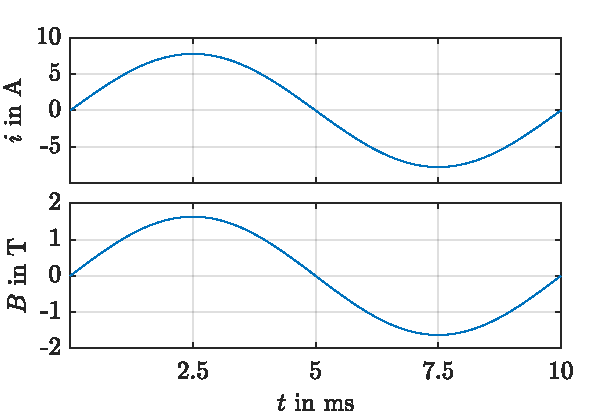
\includegraphics{ex01/solution_FluxDensity.pdf}
        \caption{Trajectories of the current $i(t)$ in the upper and the magnetic flux density $B(t)$ in the lower part of the figure.}
        \label{fig:solution_FluxDensity}
    \end{figure}

\end{solutionblock}



%%%%%%%%%%%%%%%%%%%%%%%%%%%%%%%%%%%%%%%%%%%%%%%%%%%%%%%%%%%%%

\subtask{How large is the magnetic flux linkage $\mathit{\Psi}(t)$ of the magnetic field generated by the excitation coil to the coil in the air gap?}
\begin{solutionblock}

    According to Fig.~\ref{fig:CoilSurface}, the direction of vector d$\boldsymbol{S}$ is in the opposite direction of the flux density vector $\boldsymbol{{B}}_{\updelta}$. Therefore, the flux linkage has a negative sign:
    \begin{equation}
        \psi(t) = N_{\mathrm{c}} \phi(t)
        = - N_{\mathrm{c}} A_{\mathrm{\updelta}} B_{\mathrm{\updelta}}(t).
    \end{equation}

    With the given and calculated values, the flux linkage is defined with:
    \begin{equation}
        \psi(t) = -10 \cdot (30 \cdot 30) \cdot 10^{-6} \ \si{m^2} \cdot 1.63 \ \si{T} \cdot \sin(2 \pi  \cdot 100 \ \si{Hz} \cdot t)
        = -0.0147 \ \si{Vs} \cdot \sin(2 \pi \cdot 100 \ \si{Hz} \cdot t).
    \end{equation}

\end{solutionblock}


%%%%%%%%%%%%%%%%%%%%%%%%%%%%%%%%%%%%%%%%%%%%%%%%%%%%%%%%%%%%%

\subtask{How large is the induced voltage $u_{\mathrm{i}}(t)$ of the coil in the air gap? Also, sketch the trajectory $u_{\mathrm{i}}$.}
\begin{solutionblock}
    The induced voltage is the differential of the magnetic flux linkage and therefore, defined as:
    \begin{equation}
        u_{\mathrm{i}}(t) = -\frac{\mathrm{d}\psi(t)}{\mathrm{d}t}
        = - 2 \pi f \mathit{\hat{\Psi}} \cos(2 \pi f t).
    \end{equation}

    In addition, the induced voltage is calculated with the previous calculated values:
    \begin{equation}
        u_{\mathrm{i}}(t) = -2 \pi \cdot 100 \ \si{Hz} \cdot (-0.0147 \ \si{Vs}) \cdot \cos(2 \pi \cdot 100 \ \si{Hz} \cdot t)
        = 9.2 \ \si{V} \cdot \cos(2 \pi \cdot 100 \ \si{Hz} \cdot t).
    \end{equation}

    In the upper part of Fig.~\ref{fig:solution_InducedVoltage}, the calculated current from the previous task is shown again. The induced voltage is visualized in the lower part of the figure. 
    \begin{figure}[ht]
        \centering
        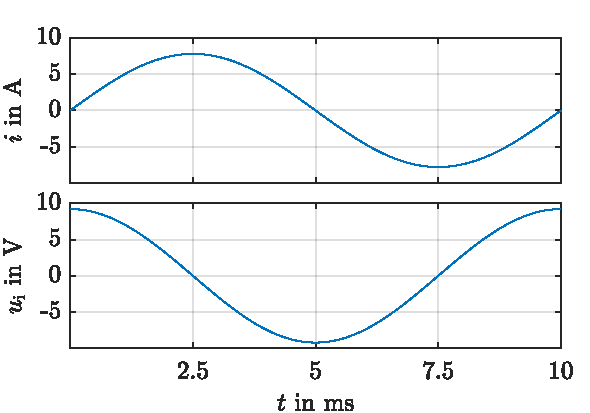
\includegraphics{ex01/solution_InducedVoltage.pdf}
        \caption{Trajectories of the current $i(t)$ in the upper and the induced voltage $u_{\mathrm{i}}(t)$ in the lower part of the figure.}
        \label{fig:solution_InducedVoltage}
    \end{figure}
    
\end{solutionblock}



%%%%%%%%%%%%%%%%%%%%%%%%%%%%%%%%%%%%%%%%%%%%%%%%%%%%%%%%%%%%%

\subtask{Calculate the mutual inductance $M$ between the excitation coil and the air gap coil.}
\begin{solutionblock}
   The mutual inductance is defined as follows:
    \begin{equation}
        M = M_{\mathrm{21}} = \frac{\psi_{\mathrm{2}}(t)}{i_{\mathrm{1}}(t)}
        = \frac{\mathit{\hat{\Psi}} \sin(2 \pi f t)}{\hat{I} \sin(2 \pi f t)}
        = \frac{\mathit{\hat{\Psi}}}{\hat{I}}
        = \frac{-0.0147 \ \si{Vs}}{7.8 \ \si{A}}
        = -1.88 \ \si{mH}.
    \end{equation}

\end{solutionblock}





%%%%%%%%%%%%%%%%%%%%%%%%%%%%%%%%%%%%%%%%%%%%%%%%%%%%%%%%%%%%%
%% Task 3 %%
%%%%%%%%%%%%%%%%%%%%%%%%%%%%%%%%%%%%%%%%%%%%%%%%%%%%%%%%%%%%%


\task{Moving current-carrying conductor in a magnetic field}
An electrical conductor (length $l$ = 1 m, resistance $R$ = 0.2 $\Omega$) is connected via two flexible supply lines from a battery (open circuit voltage $U_{\mathrm{B0}}$ = 12 V, internal resistance $R_{\mathrm{Bi}}$ = 0.1 $\Omega$) and is excited with direct current $I$. The conductor is located in an air gap between two very long permanent magnets pole pieces, that are perpendicular to the conductor axis.
The magnetic flux density directed downwards perpendicular to the conductor axis $B_{\mathrm{\updelta}}$ = 0.8 T in the air gap. The self-inductance of the conductor and the wire connections is neglected.

\begin{figure}[htb]
    \centering
    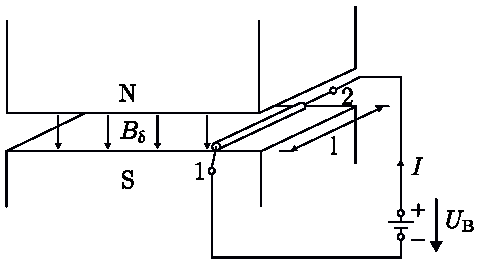
\includegraphics{ex01/ConductorInMagneticField.pdf}
    \caption{Current-carrying conductor in magnetic field.}
    \label{fig:ConductorInMagneticField}
\end{figure}


%%%%%%%%%%%%%%%%%%%%%%%%%%%%%%%%%%%%%%%%%%%%%%%%%%%%%%%%%%%%%

\subtask{Draw the electrical equivalent circuit diagram of the battery and resting conductor, and enter the direction of current flow $I$ in the load convention style. How large is $I$?}
\begin{solutionblock}
    As the magnetic field is constant over time, no induction occurs. Only the electrical battery voltage acts according to the equivalent circuit diagram in Fig.~\ref{fig:solution_EquivalentCircuitDiagram}. Hence, the current is calculated with:
    \begin{equation}
        I = \frac{U_{\mathrm{B0}}}{R_{\mathrm{Bi}}+R}
        = \frac{12 \ \si{V}}{(0.1+0.2) \ \si{\Omega}}
        = 40 \ \si{A}.
    \end{equation}

    \begin{figure}[ht]
        \centering
        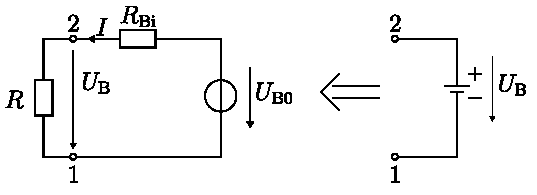
\includegraphics{ex01/solution_equivalentCircuitDiagram.pdf}
        \caption{Equivalent circuit diagram for the battery and resting conductor marked here with $R$.}
        \label{fig:solution_EquivalentCircuitDiagram}
    \end{figure}

\end{solutionblock}



%%%%%%%%%%%%%%%%%%%%%%%%%%%%%%%%%%%%%%%%%%%%%%%%%%%%%%%%%%%%%

\subtask{In which direction shows the Lorentz force $F$ on the conductor? How big is this force?}
\begin{solutionblock}
    The force $F$ acts at right angles to the field and current flow direction, this means, in the direction of the air gap surface to the right, which is shown in Fig.~\ref{fig:solution_LorentzForce}. Since the direction of current flow and field direction form a right angle with each other, the maximum possible force occurs:
    \begin{equation}
        F = I l B_{\mathrm{\updelta}}
        = 40 \ \si{A} \cdot 1 \ \si{m} \cdot 0.8 \ \si{T}
        = 32 \ \si{N}.
    \end{equation}
    
    As the conductor is flexibly connected to the battery via flexible connections the force $F$ in the air gap accelerates it to the right in its direction.

    \begin{figure}[ht]
        \centering
        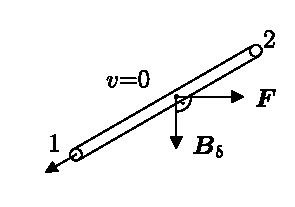
\includegraphics{ex01/solution_LorentzForce.pdf}
        \caption{Acting Lorentz force on the conductor in the air gap.}
        \label{fig:solution_LorentzForce}
    \end{figure}

\end{solutionblock}



%%%%%%%%%%%%%%%%%%%%%%%%%%%%%%%%%%%%%%%%%%%%%%%%%%%%%%%%%%%%%

\subtask{Draw the electrical equivalent circuit diagram for the combination of the moving conductor and feeding battery with the conditions at conductor side $l$. What additional electrical voltage occurs?}
\begin{solutionblock}
    If the conductor is moved by the force $F$ at the speed $v$, the movement induction in the conductor along the length $l$ creates a movement field strength against the direction of the tangent vector:
    \begin{equation}
        \boldsymbol{E}_{\mathrm{b}} = \boldsymbol{v} \times \boldsymbol{B}_{\mathrm{\updelta}}.
    \end{equation}
    
    Therefore, between 2 and 1 the voltage $u_{\mathrm{i}}$ is induced:
    \begin{equation}
        u_{\mathrm{i}}
        = \int_{2}^{1} (\boldsymbol{v} \times \boldsymbol{B}_{\updelta}) \mathrm{d}\boldsymbol{s}
        = - \int_{2}^{1} v B_{\updelta} \mathrm{d}s
        = -v B_{\updelta} l
        = U_{\mathrm{i}}.
    \end{equation}

    In the equivalent circuit diagram (Fig.~\ref{fig:solution_movingConductor}), the induced voltage acts in series with the battery voltage:
    \begin{equation}
        U_{\mathrm{B0}} + U_{\mathrm{i}} = (R_{\mathrm{Bi}} + R) I
        = U_{\mathrm{B0}} - v B_{\updelta} l.
    \end{equation}

    As long as $v B_{\updelta} l$ is less than $U_{\mathrm{B0}}$, is $I$ > 0 and the driving force $F$ > 0 remains effective. The induced voltage acts against the current direction $I$, which is the cause of the conductor movement through $F$, and therefore acts against the cause of its creation (Lenz's rule, Fig.~\ref{fig:solution_movingConductor}).

    \begin{figure}[ht]
        \centering
        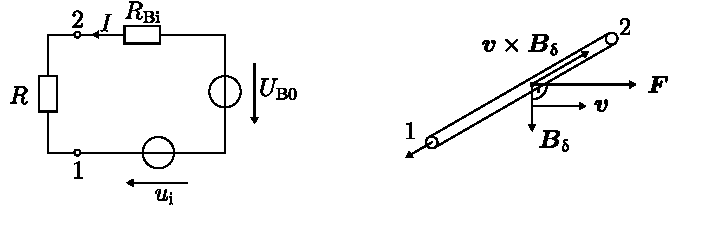
\includegraphics{ex01/solution_movingConductor.pdf}
        \caption{Moving conductor with the induced voltage $u_{\mathrm{i}}$ as an external voltage, a) equivalent electrical circuit diagram, b) direction of the Lorentz force $F$.}
        \label{fig:solution_movingConductor}
    \end{figure}

\end{solutionblock}




%%%%%%%%%%%%%%%%%%%%%%%%%%%%%%%%%%%%%%%%%%%%%%%%%%%%%%%%%%%%%

\subtask{To what final velocity $v_{\mathrm{0}}$ is the conductor in the air gap accelerated by $F$ if no mechanical braking force acts on it and if one considers the air gap as arbitrary long? How is the current $I$ in the conductor after reaching the final velocity?}
\begin{solutionblock}

    The final velocity $v_{\mathrm{0}}$ in the air gap is reached when, the sum of all forces acting on the conductor is zero ($\sum F = 0$), according to Newton's second axiom.
    Without mechanical forces from outside, this is this only true when $I$ = 0 due to $F = I l B_{\updelta}$. With the equivalent circuit from Fig.~\ref{fig:solution_movingConductor} the following equation is defined:
    \begin{equation}
        U_{\mathrm{B0}} = (R_{\mathrm{Bi}} + R) I - U_{\mathrm{i}},
    \end{equation}
    with $I$ = 0, it arranges to:
    \begin{equation}
        U_{\mathrm{B0}} = - U_{\mathrm{i}}
        = v_{\mathrm{0}} B_{\updelta} l.
    \end{equation}

    Hence, the final velocity is calculated as:
    \begin{equation}
        v_{\mathrm{0}} = \frac{U_{\mathrm{B0}}}{B_{\updelta} l}
        = \frac{12 \ \si{V}}{0.8 \ \si{T} \cdot 1 \ \si{m}}
        = 15 \ \frac{\si{m}}{\si{s}}.
    \end{equation}

    At the final speed $v_{\mathrm{0}}$, the induced voltage and battery voltage canceled each other out, such that the current $I$ is zero.

\end{solutionblock}


%%%%%%%%%%%%%%%%%%%%%%%%%%%%%%%%%%%%%%%%%%%%%%%%%%%%%%%%%%%%%

\subtask{Assume that the conductor experiences a braking force due to friction $F_{\mathrm{R}}$= 10 N. To what final velocity $v$ does the conductor now accelerate? What is the current $I$ in the conductor?}
\begin{solutionblock}
    The final velocity $v$ is reached when no further accelerating force acts on the conductor, i.e., when $F - F_{\mathrm{R}} = 0$. The force $F$ is defined as:
    \begin{equation}
        F = I l B_{\updelta}
        = F_{\mathrm{R}} = 10 \ \si{N}.
    \end{equation}
    By rearranging, the necessary current is calculated with:
    \begin{equation}
        I = \frac{10 \ \si{Nm}}{1 \ \si{m} \cdot 0.8 \ \si{T}}
        = 12.5 \ \si{A}.
    \end{equation}

    With the voltage equation again from the equivalent circuit diagram:
    \begin{equation}
        U_{\mathrm{B0}} = (R_{\mathrm{Bi}}+R)I - u_{\mathrm{i}},
    \end{equation}
    with
    \begin{equation}
        u_{\mathrm{i}} = - v B_{\updelta} l.
    \end{equation}
    Hence, the velocity $v$ calculates as follows:
    \begin{equation}
        v = \frac{U_{\mathrm{B0}}-(R_{\mathrm{Bi}}+R)I}{B_{\updelta} l}
        = \frac{12 \ \si{V} - 0.3 \ \si{\Omega} \cdot 12.5 \ \si{A}}{0.8 \ \si{T} \cdot 1 \ \si{m}}
        = 10.31 \ \frac{\si{m}}{\si{s}}.
    \end{equation}

    The Lorentz force and the friction force are visualized in Fig.~\ref{fig:solution_LorentzForce_balanceOfForces} after reaching the final speed.
    \begin{figure}[ht]
        \centering
        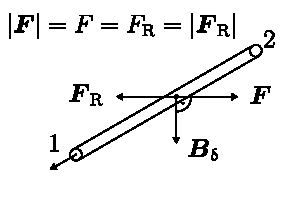
\includegraphics{ex01/solution_LorentzForce_balanceOfForces.pdf}
        \caption{Indicates the balance of forces after reaching the final speed.}
        \label{fig:solution_LorentzForce_balanceOfForces}
    \end{figure}

\end{solutionblock}



%%%%%%%%%%%%%%%%%%%%%%%%%%%%%%%%%%%%%%%%%%%%%%%%%%%%%%%%%%%%%

\subtask{What mechanical power $P_{\mathrm{m}}$ is required so that the conductor can move against the braking friction force $F_{\mathrm{R}}$ = 10 N with the final velocity $v$ determined in task 3.5. Sketch the curves $v(I)$ and $v(F)$ for a variable braking force $F_{\mathrm{R}}$ between $v_{\mathrm{0}}$ and $v$ = 0.}
\begin{solutionblock}

    The mechanical power is calculated as follows:
    \begin{equation}
        P_{\mathrm{m}} = F_{\mathrm{R}} v
        = 10 \ \si{N} \cdot 10.31 \ \si{m/s}
        = 103.1 \ \si{W}.
    \end{equation}

    The relationship between the current and the velocity is calculated with:
    \begin{equation}
        v = \frac{U_{\mathrm{B0}}-(R_{\mathrm{Bi}}+R)I}{B_{\updelta} l},
    \end{equation}
    by changing the value of the current. This results in the left part of Fig.~\ref{fig:solution_conductorSpeed}.
    The corresponding force $F$ is calculated as:
    \begin{equation}
        F = I l B_{\updelta},
    \end{equation}
    and the resulting values are shown in der right part of Fig.~\ref{fig:solution_conductorSpeed}.
    \begin{figure}[ht]
        \centering
        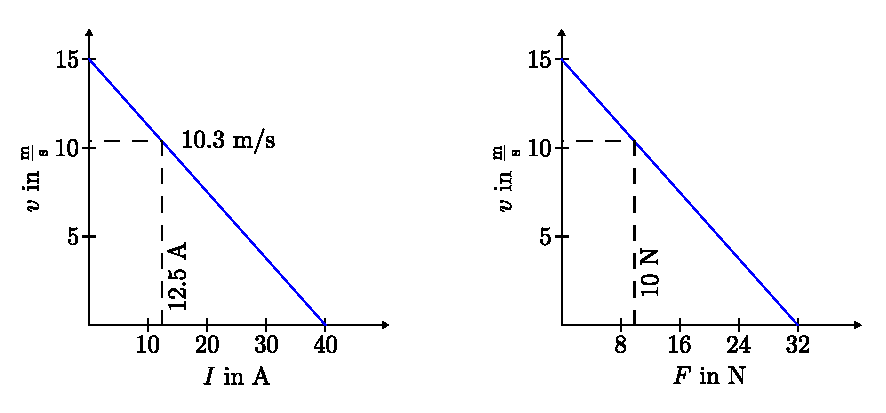
\includegraphics{ex01/solution_conductorSpeed.pdf}
        \caption{Current and force of the conductor in relationship to the velocity.}
        \label{fig:solution_conductorSpeed}
    \end{figure}

\end{solutionblock}



%%%%%%%%%%%%%%%%%%%%%%%%%%%%%%%%%%%%%%%%%%%%%%%%%%%%%%%%%%%%%

\subtask{What is the electrical power drawn from the battery $P_{\mathrm{el}}$ for the operating point from task 3.5? What is the efficiency $\eta$ and the power loss $P_{\mathrm{l}}$ when converting electrical power into mechanical power? How does the conductor act as an electromechanical energy converter?}
\begin{solutionblock}
    The electrical power for the given operating point is calculated with:
    \begin{equation}
        P_{\mathrm{el}} = U_{\mathrm{B0}} I
        = 12 \ \si{V} \cdot 12.5 \ \si{A}
        = 150 \ \si{W},
    \end{equation}
    which is used in the next step for the efficiency calculation:
    \begin{equation}
        \eta = \frac{P_{\mathrm{out}}}{P_{\mathrm{in}}}
        = \frac{P_{\mathrm{m}}}{P_{\mathrm{el}}}
        = \frac{103.1 \ \si{W}}{150 \ \si{W}}
        = 68.7 \ \si{\%}.
    \end{equation}

    The total losses are calculated as follows:
    \begin{equation}
        P_{\mathrm{l}} = P_{\mathrm{in}} - P_{\mathrm{out}}
        = 150 \ \si{W} - 103.1 \ \si{W}
        = 46.9 \ \si{W}.
    \end{equation}

    The conductor moves against the braking external frictional force $F_{\mathrm{R}}$, hence, it acts as a motor. It converts electrical energy from the battery into mechanical energy.

\end{solutionblock}


    %%%%%%%%%%%%%%%%%%%%%%%%%%%%%%%%%%%%%%%%%%%%%%%%%%%%%%%%%%%%%
%% Begin exercise %%
%%%%%%%%%%%%%%%%%%%%%%%%%%%%%%%%%%%%%%%%%%%%%%%%%%%%%%%%%%%%%
\ex{DC machine}


\normalsize{\textbf{Acknowledgement}: The following exercise is adapted from ``Elektrische Maschinen und Antriebe Übungsbuch: Aufgapen mit Lösungsweg'' by A. Binder, Springer, 2017}\\



%%%%%%%%%%%%%%%%%%%%%%%%%%%%%%%%%%%%%%%%%%%%%%%%%%%%%%%%%%%%%
%% Task 1 %%
%%%%%%%%%%%%%%%%%%%%%%%%%%%%%%%%%%%%%%%%%%%%%%%%%%%%%%%%%%%%%

\task{Six-pole loop winding}
A six-pole DC machine with an axial laminated core length $l_{\mathrm{z}}$ = 120 mm and a internal stator diameter $d_{\mathrm{s}}$ = 190 mm has an ideal pole coverage $\alpha$ = 0.7 and a maximum radial magnetic air gap flux density $\hat{B}_{\updelta}$ = 0.85 T at no-load. The armature of the machine is equipped with a two-layer lap winding with a coil winding number $N_{\mathrm{c}}$ = 20 and $K$ = 31 commutator segments.
The machine has a interpole winding connected in series with the armature winding to improve commutation. The total resistance of the armature and interpole winding is $\Ra$ = 0.14 $\Omega$.


%%%%%%%%%%%%%%%%%%%%%%%%%%%%%%%%%%%%%%%%%%%%%%%%%%%%%%%%%%%%%
\subtask{What is the total number $z_{\mathrm{a}}$ of armature conductors?}

\begin{solutionblock}
    The total number is calculated as follows
    \begin{equation}
        z_{\mathrm{a}} = 2 K N_{\mathrm{c}}
        = 2 \cdot 31 \cdot 20
        = 1240,
    \end{equation}
    with $K$ number of commutator elements and $N_{\mathrm{c}}$ number of conductor turns per coil.

\end{solutionblock}


%%%%%%%%%%%%%%%%%%%%%%%%%%%%%%%%%%%%%%%%%%%%%%%%%%%%%%%%%%%%%
\subtask{Calculate the induced voltage $\Ui$ at a rotational speed of $n$ = 4000 1/min.}

\begin{solutionblock}
    First, the pole pitch is calculated with
    \begin{equation}
        \taup = \frac{d_{\mathrm{s}} \pi}{2 p}
        = \frac{190 \ \si{mm} \cdot \pi}{6}
        = 99.5 \ \si{mm},
    \end{equation}
    where $d_{\mathrm{s}}$ is the inner stator diameter and $p$ the pole pair number.

    The induced voltage per armature conductor calculates as
    \begin{equation}
        U_{\mathrm{i,c}} = \frac{\mu_{\mathrm{0}} N_{\mathrm{f}} \lz d_{\mathrm{a}}}{2 \delta p} I_{\mathrm{f}} \omega,
    \end{equation}
    with $N_{\mathrm{f}}$ field conductor loops and the air gap length $\delta$.

    The total induced voltage is defined with
    \begin{equation}
        U_{\mathrm{i}} = \frac{N_{\mathrm{a}} \alpha}{2a} U_{\mathrm{i,c}},
    \end{equation}
    with $N_{\mathrm{a}}$ armature conductor loops and the pole coverage $\alpha$.
    For the lap winding, the number of parallel winding branches $2a$ is equal to the number of the magnetic poles $2p$, that leads to $a$ = 3.
    
    Hence, the total induced voltage is calculated by
    \begin{equation}
        U_{\mathrm{i}} = \omega I_{\mathrm{f}} \frac{\mu_{\mathrm{0}} \alpha N_{\mathrm{f}} N_{\mathrm{a}} \lz \taup}{2 \pi \delta a},
    \end{equation}
    with
    \begin{equation}
        \hat{B_{\updelta}} = \frac{\mu_{\mathrm{0}} N_{\mathrm{f}}}{2 \delta p} I_{\mathrm{f}},
        \label{eq:B_hat_task1}
    \end{equation}
    resulting in
    \begin{align}
        \begin{split}
            U_{\mathrm{i}} &= \hat{B_{\updelta}} \omega \frac{\alpha N_{\mathrm{a}} \lz \taup p}{\pi a}\\
            &= 0.85 \ \si{T} \cdot 2\pi \frac{4000}{60} \ \si{\frac{1}{s}} \cdot \frac{0.7 \cdot \frac{1240}{2} \cdot 0.12 \ \si{m} \cdot 0.0995 \ \si{m} \cdot 3}{\pi \cdot 3}
            = 587.3 \ \si{V},
        \end{split}
    \end{align}
    where $l_{\mathrm{z}}$ is the length of the machine and $\hat{B}_{\updelta}$ the maximum flux density in the air gap.
    

\end{solutionblock}




%%%%%%%%%%%%%%%%%%%%%%%%%%%%%%%%%%%%%%%%%%%%%%%%%%%%%%%%%%%%%
\subtask{The machine operates as a motor. For this purpose, a voltage of $\Ua$ = 600 V is applied. How large is the armature current $\Ia$?}


\begin{solutionblock}
    Derived from the equivalent circuit diagram, the voltage equation is given with:
    \begin{equation}
        \Ua = \Ui + \Ia \Ra.
    \end{equation}

    The above equation is resorted and solved for the armature current as follows:
    \begin{equation}
        \Ia = \frac{\Ua - \Ui}{\Ra}
        = \frac{\left(600 - 587.3\right) \si{V}}{0.14 \ \si{\Omega}}
        = 90.8 \ \si{A}.
    \end{equation}

\end{solutionblock}


%%%%%%%%%%%%%%%%%%%%%%%%%%%%%%%%%%%%%%%%%%%%%%%%%%%%%%%%%%%%%
\subtask{Calculate the Lorentz force per conductor $F_{\mathrm{c}}$ and per pole $F_{\mathrm{pole}}$. Calculate in addition the resulting average electromagnetic torque $T$. An air gap of $\delta$~=~1 mm is assumed.}

\begin{solutionblock}
    The current per armature conductor is calculated with:
    \begin{equation}
        I_{\mathrm{c}} = \frac{\Ia}{2a}
        = \frac{90.8 \ \si{A}}{6}
        = 15.13 \ \si{A}.
    \end{equation}

    The Lorentz force per armature conductor is determined as:
    \begin{equation}
        F_{\mathrm{c}} = \hat{B}_{\updelta} \lz I_{\mathrm{c}}
        = 0.85 \ \si{T} \cdot 0.12 \ \si{m} \cdot 15.13 \ \si{A}
        = 1.54 \ \si{N}.
    \end{equation}

    With $F_{\mathrm{c}}$ the Lorentz force per pol is calculated with:
    \begin{equation}
        F_{\mathrm{pole}} = \alpha \frac{\za}{2p} F_{\mathrm{c}}
        = 0.7 \cdot \frac{1240}{6} \cdot 1.54 \ \si{N}
        = 222.8 \ \si{N}.
    \end{equation}


    The torque per conductor is defined as follows 
    \begin{equation}
        T_{\mathrm{c}} = F_{\mathrm{c}} \frac{d_{\mathrm{a}}}{2}
        = \frac{\mu_{\mathrm{0}} N_{\mathrm{f}} \lz d_{\mathrm{a}}}{8\delta p a} I_{\mathrm{f}}I_{\mathrm{a}},
    \end{equation}
    with the outer armature diameter $d_{\mathrm{a}} = d_{\mathrm{s}} - 2\delta$.

    Hence, the resulting average torque is given as
    \begin{equation}
        T = 2 \alpha N_{\mathrm{a}} T_{\mathrm{c}}
        = \frac{\mu_{\mathrm{0}} \alpha N_{\mathrm{f}} N_{\mathrm{a}} \lz d_{\mathrm{a}}}{4 \delta p a} I_{\mathrm{f}} I_{\mathrm{a}},
    \end{equation}
    with \eqref{eq:B_hat_task1} resulting in the following equation
    \begin{align}
        \begin{split}
            T &= \hat{B_{\updelta}} \frac{\alpha N_{\mathrm{a}} \lz d_{\mathrm{a}}}{2a} \Ia\\
            &= 0.85 \ \si{T} \cdot \frac{0.7 \cdot \frac{1240}{2} \cdot 0.12 \ \si{m} \cdot 0.188 \ \si{m}}{2 \cdot 3} \cdot 90.8 \ \si{A}
            = 125.9 \ \si{Nm}.
        \end{split}
    \end{align}

   

\end{solutionblock}



%%%%%%%%%%%%%%%%%%%%%%%%%%%%%%%%%%%%%%%%%%%%%%%%%%%%%%%%%%%%%
\subtask{Calculate the motor losses. Assume that the iron losses and friction losses can be neglected as well as that the field excitation is produced via permanent magnets.}


\begin{solutionblock}
    Based on the assumptions, only the ohmic losses occur in the machine:
    \begin{equation}
        \Pl = \Pcu = \Ra I_{\mathrm{a}}^2
        = 0.14 \ \si{\Omega} \cdot \left(90.8 \ \si{A} \right)^2
        = 1154.2 \ \si{W}.
    \end{equation}
   

\end{solutionblock}




%%%%%%%%%%%%%%%%%%%%%%%%%%%%%%%%%%%%%%%%%%%%%%%%%%%%%%%%%%%%%
\subtask{Calculate the efficiency $\eta$ for the given operating point.}

\begin{solutionblock}

    The electric power is defined with
    \begin{equation}
        P_{\mathrm{el}} = \Ua \Ia
        = 600 \ \si{V} \cdot 90.8 \ \si{A}
        = 54480 \ \si{W},
    \end{equation}
    and the mechanical output power as:
    \begin{equation}
        P_{\mathrm{mech}} = T \omega 
        = 125.9 \ \si{Nm} \cdot 2 \pi \cdot \frac{4000}{60} \ \si{\frac{1}{s}}
        = 52753\ \si{W}.
    \end{equation}

    The efficiency results in:
    \begin{equation}
        \eta = \frac{P_{\mathrm{mech}}}{P_{\mathrm{el}}}
        = \frac{52753 \ \si{W}}{54480 \ \si{W}}
        = 96.8 \ \%.
    \end{equation}
\end{solutionblock}



%%%%%%%%%%%%%%%%%%%%%%%%%%%%%%%%%%%%%%%%%%%%%%%%%%%%%%%%%%%%%
%% Task 2 %%
%%%%%%%%%%%%%%%%%%%%%%%%%%%%%%%%%%%%%%%%%%%%%%%%%%%%%%%%%%%%%

\task{Design parameters of a DC machine}
The separately-excited four-pole DC machine with a two-layer lap winding has a stator with the diameter of $d_{\mathrm{s}}$ = 133 mm and a length of $\lz$ = 80 mm.
The armature has $Q$ = 30 slots, $u$ = 3 commutators per slot and layer as well as $N_{\mathrm{c}}~$=~9 windings per armature coil.
The maximum air gap flux density is $\hat{B}_{\updelta}$~=~0.9 T, the ideal pole coverage is $\alpha$ = 0.7, and, the air gap width is $\delta$~=~1.5~mm.
The nominal speed of the machine is $\nN$ = 1440 $\mathrm{min}^{-1}$, with an armature current of $I_{\mathrm{a,n}}$~=~22 A. The excitation values are given with $I_{\mathrm{f}}$ = 0.5 A and $U_{\mathrm{f}}$ = 230 V.



%%%%%%%%%%%%%%%%%%%%%%%%%%%%%%%%%%%%%%%%%%%%%%%%%%%%%%%%%%%%%
\subtask{What is the pole pitch $\tau_{\mathrm{p}}$ and the flux per pole $\phi_{\mathrm{\updelta}}$?}

\begin{solutionblock}
    The pole pitch calculates as follows
    \begin{equation}
        \tau_{\mathrm{p}} = \frac{d_{\mathrm{s}} \pi}{2 p}
        = \frac{133 \ \si{mm} \cdot \pi}{4}
        = 104.5 \ \si{mm},
    \end{equation}
    with the inner stator diameter $d_{\mathrm{s}}$ and the pole pair number $p$ = 2.
    The flux per pole is calculated as
    \begin{equation}
        \phiDelta = \alpha \tau_{\mathrm{p}} \lz \hat{B}_{\updelta}
        = 0.7 \cdot 0.1045 \ \si{m} \cdot 0.08 \ \si{m} \cdot 0.9 \ \si{T}
        = 5.265 \ \si{mWb},
    \end{equation}
    where $\alpha$ represents the pole coverage, $l_{\mathrm{z}}$ is the axial length of the machine and the maximum flux density $\hat{B_{\updelta}}$ in the air gap.

\end{solutionblock}


%%%%%%%%%%%%%%%%%%%%%%%%%%%%%%%%%%%%%%%%%%%%%%%%%%%%%%%%%%%%%
\subtask{What is the number of commutator elements $K$, the total number of armature conductors $\za$ and the number of parallel armature branches $2a$.}

\begin{solutionblock}
    The number of commutator elements is calculated as
    \begin{equation}
        K = Q u
        = 30 \cdot 3
        = 90,
    \end{equation}
    with $Q$ slots and the slot to commutator ration $u$. 
    The total number of armature conductors is defined by
    \begin{equation}
        \za = 2 K N_{\mathrm{c}}
        = 2 \cdot 90 \cdot 9
        = 1620,
    \end{equation}
    with $K$ number of commutator elements and $N_{\mathrm{c}}$ number of conductor turns per coil.

    For a lap winding, the number of poles are directly connected with the number of parallel branches, which results in:
    \begin{equation}
        2a = 2p = 4.
    \end{equation}
\end{solutionblock}



%%%%%%%%%%%%%%%%%%%%%%%%%%%%%%%%%%%%%%%%%%%%%%%%%%%%%%%%%%%%%
\subtask{Determine the induced voltage $\Ui$ at nominal speed $\nN$ and the electromagnetic torque $\Tn$. What is the necessary armature voltage $\Uan$ during motor operation mode, when $\Ra$ = 1 $\Omega$? How large is the motor output power, neglecting the friction and the soft magnetic material losses (hysteresis + eddy current)? Determine the no-load rotational speed $\nO$ at the fixed flux $\phiDelta$.}

\begin{solutionblock}
    The induced voltage is calculated by
    \begin{equation}
        U_{\mathrm{i}} = \omega I_{\mathrm{f}} \frac{\mu_{\mathrm{0}} \alpha N_{\mathrm{f}} N_{\mathrm{a}} \lz \taup}{2 \pi \delta a},
    \end{equation}
    with
    \begin{equation}
        \hat{B_{\updelta}} = \frac{\mu_{\mathrm{0}} N_{\mathrm{f}}}{2 \delta p} I_{\mathrm{f}},
        \label{eq:B_hat_task2}
    \end{equation}
    resulting in
    \begin{align}
        \begin{split}
            U_{\mathrm{i}} &= \hat{B_{\updelta}} \omega \frac{\alpha N_{\mathrm{a}} \lz \taup p}{\pi a}\\
            &= 0.9 \ \si{T} \cdot 2\pi \frac{1440}{60} \ \si{\frac{1}{s}} \cdot \frac{0.7 \cdot \frac{1620}{2} \cdot 0.08 \ \si{m} \cdot 0.1045 \ \si{m} \cdot 2}{\pi \cdot 2}
            = 204.8 \ \si{V}.
        \end{split}
    \end{align}

    The average torque is given as
    \begin{equation}
        \Tn
        = \frac{\mu_{\mathrm{0}} \alpha N_{\mathrm{f}} N_{\mathrm{a}} \lz d_{\mathrm{a}}}{4 \delta p a} I_{\mathrm{f}} I_{\mathrm{a}},
    \end{equation}
    with \eqref{eq:B_hat_task2} resulting in the following equation
    \begin{align}
        \begin{split}
            T &= \hat{B_{\updelta}} \frac{\alpha N_{\mathrm{a}} \lz d_{\mathrm{a}}}{2a} \Ia\\
            &= 0.9 \ \si{T} \cdot \frac{0.7 \cdot \frac{1620}{2} \cdot 0.08 \ \si{m} \cdot 0.130 \ \si{m}}{2 \cdot 2} \cdot 22 \ \si{A}
            = 29.2 \ \si{Nm}.
        \end{split}
    \end{align}

    The armature voltage $\Uan$ at nominal speed is derived from the equivalent circuit diagram and therefore given with:
    \begin{equation}
        \Uan = \Ui + \Ra \In
        = 204.8 \ \si{V} + 1 \ \si{\Omega} \cdot 22 \ \si{A}
        = 226.8 \ \si{V}.
    \end{equation}

    The mechanical output power is defined with:
    \begin{equation}
        P_{\mathrm{mech}} = \Tn \omega
        = 29.2 \ \si{Nm} \cdot 2\pi \cdot \frac{1440}{60} \ \si{\frac{1}{s}}
        = 4403 \ \si{W}.
    \end{equation}

    To calculate the maximum speed at no-load, the friction and soft magnetic losses are neglected. Therefore, the armature current is assumed to zero ($\Ia$ = 0) resulting in $U_{\mathrm{i}} = \Ua$.
    Hence, the voltage equation is given with:
    \begin{equation}
        \Ui = \Ua = \hat{B_{\updelta}} \omega \frac{\alpha N_{\mathrm{a}} \lz \taup p}{\pi a}.
    \end{equation}

    By rearranging the equation from above, the no-load speed is calculated as follows:
    \begin{equation}
        n = \frac{\Ua \pi a}{\hat{B_{\updelta}} \alpha N_{\mathrm{a}} \lz \taup p 2\pi}
        = \frac{226.8 \ \si{V} \cdot \pi \cdot 2}{0.9 \ \si{T} \cdot 0.7 \cdot \frac{1620}{2} \cdot 0.08 \ \si{m} \cdot 0.1045 \ \si{m} \cdot 2 \cdot 2\pi}
        = 26.8 \ \si{\frac{1}{s}} = 1607 \ \si{\frac{1}{min}}.
    \end{equation}

\end{solutionblock}



%%%%%%%%%%%%%%%%%%%%%%%%%%%%%%%%%%%%%%%%%%%%%%%%%%%%%%%%%%%%%
\subtask{How many brush pairs does the machine have? How big is the current per  brush? What is the circumferential speed of the armature under consideration of $\delta$?}

\begin{solutionblock}
    The machine has two brush pairs to meet the pole pair number, which are electrical parallel connected.
    
    At the nominal operation point, the current per brush is calculated as follows
    \begin{equation}
        I_{\mathrm{b}} = \frac{I_{\mathrm{a,n}}}{a}
        = \frac{22 \ \si{A}}{2}
        = 11 \ \si{A},
    \end{equation}
    with $a = p = 2$ due to the lap winding.

    The outer diameter of the armature is determined with
    \begin{equation}
        d_{\mathrm{a}} = d_{\mathrm{s}} - 2 \delta
        = 133 \ \si{mm} - 2 \cdot 1.5 \ \si{mm}
        = 130 \ \si{mm},
    \end{equation}

    and therefore, the circumferential speed of the armature calculates with:
    \begin{equation}
        v_{\mathrm{a}} = d_{\mathrm{a}} \pi \nN
        = 0.13 \ \si{m} \cdot \pi \cdot \frac{1440}{60} \ \si{\frac{1}{s}}
        = 9.8 \ \si{\frac{m}{s}}
        = 35.3 \ \si{\frac{km}{h}}.
    \end{equation}

\end{solutionblock}

%%%%%%%%%%%%%%%%%%%%%%%%%%%%%%%%%%%%%%%%%%%%%%%%%%%%%%%%%%%%%
\subtask{Determine the necessary excitation with ideal iron path ($\mu_{\mathrm{r}}\rightarrow \infty$) per pole. What is the number of necessary windings for each of the four coils of the excitation of the stator. Considering a real motor, is the excitation larger or smaller?}

\begin{solutionblock}
    The total field is calculated as follows
    \begin{equation}
        \theta_{\mathrm{f}} = \hat{H}_{\updelta} \delta
        = \frac{\hat{B_{\updelta}}}{\mu_{\mathrm{0}}} \delta
        = \frac{0.9 \ \si{T}}{4\pi \cdot 10^{-7} \ \si{\frac{Vs}{Am}}} \cdot 0.0015 \ \si{m}
        = 1074.3 \ \si{A},
    \end{equation}
    with the magnetic field strength $H_{\updelta}$ in the air gap. The relationship between the total excitation and the excitation per pole is
    \begin{equation}
        \theta_{\mathrm{f}} = N_{\mathrm{f,pole}} I_{\mathrm{f}},
    \end{equation}
    which results in the necessary windings per pole
    \begin{equation}
        N_{\mathrm{f,pole}} = \frac{\theta_{\mathrm{f}}}{I_{\mathrm{f}}}
        = \frac{1074.3 \ \si{A}}{0.5 \ \si{A}}
        = 2148.6,
    \end{equation}
    with the field current $I_{\mathrm{f}}$. This results in 2149 necessary turns.

    By considering iron saturation $\mu_{\mathrm{r}}$ is not constant anymore, see therefore the magnetization curves from the lecture.
    This results in lower value of $\mu_{\mathrm{r}}$ compared to the previous assumption in this task ($\mu_{\mathrm{r}}\rightarrow \infty$) and therefore the effective magnetic reluctance along the field excitation path increases. To overcome this and to provide the same effective excitation field, the field winding's MMF need to be increased by additional winding turns compared to the previous calculation.

\end{solutionblock}


%%%%%%%%%%%%%%%%%%%%%%%%%%%%%%%%%%%%%%%%%%%%%%%%%%%%%%%%%%%%%
\subtask{Determine the efficiency $\eta_{\mathrm{a}}$ of the armature and the resulting total efficiency $\eta$. Are these losses larger or smaller for real motors? Why? Give an explanation.} 

\begin{solutionblock}
    The electrical input power is calculated as follows:
    \begin{equation}
        P_{\mathrm{el,a}} = \Ua I_{\mathrm{a,n}}
        = 226.8 \ \si{V} \cdot 22 \ \si{A}
        = 4990 \ \si{W}.
    \end{equation}
    Hence, the armature efficiency is determined with:
    \begin{equation}
        \eta_{\mathrm{a}} = \frac{P_{\mathrm{mech}}}{P_{\mathrm{el,a}}}
        = \frac{4503 \ \si{W}}{5031.4 \ \si{W}}
        = 0.895
        = 89.5 \ \%.
    \end{equation}

    The field losses are calculated as
    \begin{equation}
        P_{\mathrm{el,f}} = U_{\mathrm{f}} I_{\mathrm{f}}
        = 230 \ \si{V} \cdot 0.5 \ \si{A}
        = 115 \ \si{W},
    \end{equation}
    which leads to the total efficiency:
    \begin{equation}
        \eta = \frac{P_{\mathrm{mech}}}{P_{\mathrm{el,a}}+P_{\mathrm{el,f}}}
        = \frac{4403 \ \si{W}}{4990 \si{W} + 115 \ \si{W}}
        = 0.862
        = 86.2 \ \%.
    \end{equation}

    The real losses are higher due to the air and bearing friction as well as the soft magnetic material losses (hysteresis + eddy current) which have been neglected in the above model calculation but which are present in a real machine.
\end{solutionblock}



%%%%%%%%%%%%%%%%%%%%%%%%%%%%%%%%%%%%%%%%%%%%%%%%%%%%%%%%%%%%%
\subtask{The motor should be operated with a constant armature voltage of $\Uan$ = 230 V in the flux-weakening range with $T$ = 15 Nm. What is the flux per pole $\phi_{\mathrm{pole}}$ and the armature current $\Ia$? How large is the resulting efficiency $\eta$, if the utilized iron shows no saturation and required field weakening is reached through reducing the field voltage $U_{\mathrm{f}}$.}


\begin{solutionblock}
    The armature voltage is calculated as
    \begin{equation}
        \Ua = \Ui + \Ra \Ia
        = \omega \psi_{\mathrm{f}}' + \Ra I_{\mathrm{a}},
    \end{equation}
    with $\Ia = \frac{T}{\psi_{\mathrm{f}}'}$ resulting in:
    \begin{equation}
        \Ua = \omega \psi_{\mathrm{f}}' + \frac{\Ra T}{\psi_{\mathrm{f}}'}.
    \end{equation}
    This equation is reformed to the following
    \begin{equation}
        \left(\psi_{\mathrm{f}}' \right)^2 - \frac{U_{\mathrm{a}}}{\omega} \psi_{\mathrm{f}}' + \frac{\Ra Tn}{\omega} = 0,
    \end{equation}
    which represents a quadratic equation, that is solved in the following form:
    \begin{equation}
        x^2 + P x + Q = 0.
    \end{equation}

    The solution is given as follows
    \begin{equation}
        x_{\mathrm{1,2}} = -\frac{P}{2} \pm \sqrt{\left(\frac{P}{2}\right)^2 - Q},
    \end{equation}
    with 
    \begin{equation}
        P = -\frac{U_{\mathrm{a}}}{\omega},
    \end{equation}
    which is applied according to the equation:
    \begin{equation}
        \frac{P}{2} = - \frac{230 \ \si{V}}{4 \pi \cdot \frac{1900}{60} \ \si{\frac{1}{s}}}
        = 0.578 \ \si{Vs}.
    \end{equation}

    The parameter $Q$ is defined by:
    \begin{equation}
        Q = \frac{\Ra \Tn}{\omega}
        = \frac{1 \ \si{\Omega} \cdot 15 \ \si{Nm}}{2 \pi \cdot \frac{1900}{60} \ \si{\frac{1}{s}}}
        = 0.0754 \ \si{(Vs)^2}.
    \end{equation}


    Hence, the solution is calculated as follows
    \begin{align}
        \begin{split}
            \left(\psi_{\mathrm{f}}' \right)_{\mathrm{1,2}}
            &= \frac{U_{\mathrm{a}}}{2 \omega} \pm \sqrt{\left( \frac{U_{\mathrm{a}}}{2 \omega}\right) - \frac{\Ra \Tn}{\omega}}, \\
            \left(\psi_{\mathrm{f}}' \right)_{\mathrm{1,2}}
            &= 0.578 \pm \sqrt{\left(0.578 \si{Vs} \right)^2 - 0.0754 \ \si{Vs}},
        \end{split}
    \end{align}

    with two possible solution due to the quadratic equation. Therefore, both solutions must be evaluated, starting with $\left(\psi_{\mathrm{f}}' \right)_{\mathrm{1}}$ = 0.07 Vs. The corresponding current is calculated by:
    \begin{equation}
        I_{\mathrm{a}} = \frac{\Tn}{\left(\psi_{\mathrm{f}}' \right)_{\mathrm{1}}}
        = \frac{15 \ \si{Nm}}{0.07 \ \si{Vs}}
        = 214.3 \ \si{A}.
    \end{equation}

    Testing the second solution $\left(\psi_{\mathrm{f}}' \right)_{\mathrm{2}}$ = 1.09 Vs results in
    \begin{equation}
        I_{\mathrm{a}} = \frac{\Tn}{\left(\psi_{\mathrm{f}}' \right)_{\mathrm{2}}}
        = \frac{15 \ \si{Nm}}{1.09 \ \si{Vs}}
        = 13.76 \ \si{A},
    \end{equation}
    which is the right solution due to the lower current.

    The corresponding flux per pole is calculated with:
    \begin{equation}
        \phi_{\mathrm{pole}} = \frac{\left(\psi_{\mathrm{f}}' \right)_2 }{\frac{z_{\mathrm{a}}}{2\pi}}
        = \frac{1.09 \ \si{Vs}}{\frac{1620}{2 \pi}}
        = 4.23 \ \si{mVs}.
    \end{equation}
    The relationship to the previously calculated flux per pole $\phi_{\updelta}$ is defined as follows
    \begin{equation}
        \frac{\phi_{\mathrm{pole}}}{\phiDelta}
        = \frac{4.23 \ \si{mVs}}{5.265 \ \si{mVs}}
        = 0.803
        = 80.3 \ \%.
    \end{equation}

    In the following, the armature current is set in relation to the nominal current as:
    \begin{equation}
        \frac{I_{\mathrm{a}}}{I_{\mathrm{a,n}}}
        = \frac{13.76 \ \si{A}}{22 \ \si{A}}
        = 0.63
        = 63 \ \%.
    \end{equation}

    Hence, the electrical input power is calculated with
    \begin{equation}
        P_{\mathrm{el,a}} = U_{\mathrm{a}} \Ia
        = 230 \ \si{V} \cdot 13.76 \ \si{A}
        = 3164.8 \ \si{W},
    \end{equation}
    and the mechanical power with the given values in the task description by:
    \begin{equation}
        P_{\mathrm{mech}} = T \omega
        = 15 \ \si{Nm} \cdot 2 \pi \cdot \frac{1900}{60} \ \si{\frac{1}{s}}
        = 2984.5 \ \si{W}.
    \end{equation}

    The given operating point is located in the flux-weakening range and, therefore, the excitation values and the corresponding losses are changed.
    This leads to lower excitation losses as follows
    \begin{equation}
        \frac{P_{\mathrm{el,f}}}{P_{\mathrm{el,f,n}}}
        = \frac{R_{\mathrm{f}} I^2_{\mathrm{f}}}{R_{\mathrm{f}} I^2_{\mathrm{f,n}}}
        = \frac{I^2_{\mathrm{f}}}{I^2_{\mathrm{f,n}}},
    \end{equation}
    with
    \begin{equation}
        \frac{\phi_{\mathrm{pole}}}{\phi_{\updelta}}
        = \frac{I^2_{\mathrm{f}}}{I^2_{\mathrm{f,n}}}
        = 0.803^2.
    \end{equation}

    This results in:
    \begin{equation}
        P_{\mathrm{el,f}} = P_{\mathrm{el,f,n}} \left( \frac{I_{\mathrm{f}}}{I_{\mathrm{f,n}}} \right)^2
        = 115 \ \si{W} \cdot \left(0.803 \right)^2
        = 74.2 \ \si{W}.
    \end{equation}

    The efficiency is given by:
    \begin{equation}
        \eta = \frac{P_{\mathrm{mech}}}{P_{\mathrm{el,a}} + P_{\mathrm{el,f}}}
        = \frac{2984.5 \ \si{W}}{3164.8 \ \si{W} + 74.2 \ \si{W}}
        = 0.921 = 92.1 \ \%.
    \end{equation}

\end{solutionblock}




%%%%%%%%%%%%%%%%%%%%%%%%%%%%%%%%%%%%%%%%%%%%%%%%%%%%%%%%%%%%%
%% Task 3 %%
%%%%%%%%%%%%%%%%%%%%%%%%%%%%%%%%%%%%%%%%%%%%%%%%%%%%%%%%%%%%%

\task{Submarine with DC machine}
A four-pole DC machine on the board of a submarine with $U_{\mathrm{a,n}}$ = 440 V, $\Pn$ = 65 kW, $\nN$~=~1300~$\mathrm{min^{-1}}$ has an efficiency of $\eta_{\mathrm{n}}$ = 0.9. The total losses $\Pl$ are separated in the ohmic losses $\Pcu$ in the armature with 75 \% and the soft magnetic material, friction, and additional losses ($\Pfe$ + $P_{\mathrm{fr+add}}$) with 25 \% of the total losses $\Pl$. The field excitation losses are neglected in the following.



%%%%%%%%%%%%%%%%%%%%%%%%%%%%%%%%%%%%%%%%%%%%%%%%%%%%%%%%%%%%%
\subtask{Calculate the armature current $I_{\mathrm{a,n}}$, the torque $\Tn$, the losses $P_{\mathrm{Cu,a}}$ and $P_{\mathrm{fr+add}}$, the armature winding resistance $R_{\mathrm{a}}$ and the no-load speed $n_{\mathrm{0}}$.}


\begin{solutionblock}
    The armature current calculates as follows
    \begin{equation}
        I_{\mathrm{a,n}} = \frac{\Pn / \eta_{\mathrm{n}}}{\Uan}
        = \frac{65 \ \si{kW} / 0.9}{440 \ \si{V}}
        = 164.1 \ \si{A},
    \end{equation}
    with a nominal mechanical power of $\Pn$, the efficiency $\eta_{\mathrm{n}}$ and the voltage $\Uan$.
    Hence, the torque is determined with:
    \begin{equation}
        \Tn = \frac{\Pn}{\omega_{\mathrm{n}}} 
        = \frac{65 \ \si{kW}}{2 \pi \cdot \frac{1300}{60} \ \si{\frac{1}{s}}}
        = 477.5 \ \si{Nm}.
    \end{equation}

    The efficiency is given with
    \begin{equation}
        \eta_{\mathrm{n}} = \frac{\Pn}{\Pn + \Pl},
    \end{equation}
    where $\Pl$ are the losses of the machine. To calculate them, the equation is rearranged as follows:
    \begin{equation}
        \Pl = \left(\frac{1}{\eta_{n}} - 1 \right) \Pn
        = \left(\frac{1}{0.9}-1 \right) \cdot 65\ \si{kW}
        = 7222 \ \si{W}.
    \end{equation}

    As described in the task, the cupper losses are defined by
    \begin{equation}
        P_{\mathrm{Cu,a}} = 0.75 \Pl
        = 0.75 \cdot 7222 \ \si{W} 
        = 477.5 \ \si{W},
    \end{equation}
    and, therefore, the other losses yield as follows:
    \begin{equation}
        P_{\mathrm{Fe}} + P_{\mathrm{fr + add}} = 0.25 \Pl 
        = 0.25 \cdot 7222 \ \si{W}
        = 1805.5 \ \si{W}.
    \end{equation}

    The resistance of the armature calculates with
    \begin{equation}
        P_{\mathrm{Cu,a}} = \Ra I_{\mathrm{a,n}}^{2},
    \end{equation}
    which is resorted to the following:
    \begin{equation}
        \Ra = \frac{P_{\mathrm{Cu,a}}}{I_{\mathrm{a,n}}^{2}}
        = \frac{5416.7 \ \si{W}}{\left(164.1 \ \si{A}\right)^2}
        = 0.201 \ \si{\Omega}.
    \end{equation}

    The voltage is determined according to the equivalent circuit diagram by
    \begin{equation}
        \Ua = \Ui + \Ra I_{\mathrm{a,n}},
    \end{equation}

    and, therefore, the induced voltage is calculated with
    \begin{equation}
        \Ui = \Ua - \Ra I_{\mathrm{a,n}}
        = 440 \ \si{V} - 0.201 \ \si{\Omega} \cdot 164.1 \ \si{A}
        = 407 \ \si{V}.
    \end{equation}

    In addition, the induced voltage is defined as
    \begin{equation}
        \Ui = \omega \psi_\mathrm{f}',
    \end{equation}
    which is used to calculate the flux linkage as follows:
    \begin{equation}
        \psi_{\mathrm{f}}' = \frac{\Ui}{\omega}
        = \frac{407 \ \si{V}}{2\pi \cdot \frac{1300}{60} \ \si{\frac{1}{s}}}
        = 2.99 \ \si{Vs}. 
    \end{equation}

    To calculate the maximum speed at no-load, the friction and soft magnetic losses are neglected. Therefore, the armature current is assumed to zero ($\Ia$ = 0) resulting in $U_{\mathrm{i}} = \Uan$, which leads to
    \begin{equation}
        \omega = \frac{\Uan}{\psi_{\mathrm{f}}'},
    \end{equation}
    resulting in
    \begin{equation}
        \nO = \frac{\Uan}{\psi_{\mathrm{f}}' 2 \pi} = \frac{440 \ \si{V}}{2.99 \ \si{Vs} \cdot 2 \pi}
        = 23.42 \ \si{\frac{1}{s}},
    \end{equation}
    which is a no-load speed of $\nO$ = 1405 $\mathrm{min^{-1}}$.

       
\end{solutionblock}


%%%%%%%%%%%%%%%%%%%%%%%%%%%%%%%%%%%%%%%%%%%%%%%%%%%%%%%%%%%%%
\subtask{Determine the value of the additional starter resistor $R_{\mathrm{d}}$, such that the start-up torque $T_{\mathrm{1}}$ at $U_{\mathrm{a}}=U_{\mathrm{a,n}}$ is limited to 150~\% of the nominal torque.}

\begin{solutionblock}
    As described in the task, the torque is set by
    \begin{equation}
        T_{\mathrm{1}} = 1.5 \Tn = \psi_{\mathrm{f}}' I_{\mathrm{a,1}},
    \end{equation}
    and at machine standstill, the voltage is defined as:
    \begin{equation}
        U_{\mathrm{a,n}} = \left(\Ra + R_{\mathrm{d}} \right) I_{\mathrm{a,1}}.
    \end{equation}

    Therefore, the starter resistor is calculated with
    \begin{equation}
        R_{\mathrm{d}} = \frac{U_{\mathrm{a,n}}}{I_{\mathrm{a,1}}} - \Ra
        = \frac{U_{\mathrm{a,n}} \psi_{\mathrm{f}}'}{1.5 \Tn}-\Ra
        = \frac{440 \ \si{V} \cdot 2.99 \ \si{Vs}}{1.5 \cdot 477.5 \ \si{Nm}}-0.201 \ \si{\Omega}
        = 1.635 \ \si{\Omega}.
    \end{equation}

    Hence, the starter current is determined with:
    \begin{equation}
        I_{\mathrm{a,1}} = \frac{1.5 \Tn}{\psi_{\mathrm{f}}'}
        = \frac{1.5 \cdot 477.5 \ \si{Nm}}{2.99 \ \si{Vs}}
        = 239.7 \ \si{A}.
    \end{equation}


\end{solutionblock}


%%%%%%%%%%%%%%%%%%%%%%%%%%%%%%%%%%%%%%%%%%%%%%%%%%%%%%%%%%%%%
\subtask{With a power electronic converter, the armature voltage $\Ua$ is reduced to 0.8 $\Uan$. How large is the rotational speed $n$ with the fixed flux $\phiDelta$ at the torque $T$ = 0.5 $\Tn$?}

\begin{solutionblock}
    The equation for the reduced armature voltage is given as follows
    \begin{equation}
        U_{\mathrm{a}} = 0.8 U_{\mathrm{a,n}}
        = \omega \psi_{\mathrm{f}}' + \Ra I_{\mathrm{a}},
    \end{equation}
    and the reduced torque results in a lower armature current, which is calculated with:
    \begin{equation}
        I_{\mathrm{a}} = \frac{0.5 \Tn}{\psi_{\mathrm{f}}'}.
    \end{equation}

    With this two equations from above, the speed is calculated below:
    \begin{align}
        \begin{split}
            n &= \frac{0.8 U_{\mathrm{a,n}} - \frac{\Ra 0.5 \Tn}{\psi_{\mathrm{f}}'}}{2 \pi \psi_{\mathrm{f}}'}
            = \frac{0.8 \cdot 440 \ \si{V} - \frac{0.201 \ \si{\Omega} \cdot 0.5 \cdot 477.5 \ \si{Nm}}{2.99 \ \si{Vs}}}{2 \pi \cdot 2.99 \ \si{Vs}}\\
            &= 17.89 \ \si{\frac{1}{s}}
            = 1073.6 \ \si{\frac{1}{min}}.
            \end{split}
    \end{align}


\end{solutionblock}


%%%%%%%%%%%%%%%%%%%%%%%%%%%%%%%%%%%%%%%%%%%%%%%%%%%%%%%%%%%%%
\subtask{After the submarine surfaced, the machine is now used as a generator to charge the batteries powering with marine diesel at the speed $\nN$ = 1530 $\mathrm{min^{-1}}$. What is the no-load induced voltage? How big is the armature voltage $\Ua$ at $\Ia$ = $I_{\mathrm{a,n}}$ ($\phi$ = $\phiDelta$)?}
    
\begin{solutionblock}
    The induced voltage is calculated with:
    \begin{equation}
        \Ui = U_{\mathrm{0}}
        = \omega \psi_{\mathrm{f}}'
        = 2 \pi \cdot \frac{1530}{60} \si{\frac{1}{s}} \cdot 2.99 \ \si{Vs}
        = 478.7 \ \si{V}.
    \end{equation}

    To determine the armature voltage, the ohmic voltage drop is taken into account as given below: 
    \begin{equation}
        U_{\mathrm{a}} = U_{\mathrm{0}} - I_{\mathrm{a,n}} \Ra
        = 478.7 \ \si{V} - 164.1 \ \si{A} \cdot 0.201 \ \si{\Omega}
        = 445.8 \ \si{V}.
    \end{equation}
\end{solutionblock}



%%%%%%%%%%%%%%%%%%%%%%%%%%%%%%%%%%%%%%%%%%%%%%%%%%%%%%%%%%%%%
\subtask{How large is the voltage $\Ua$ at $\phi$ = 0.7 $\phiDelta$ and $\Ia = I_{\mathrm{a,n}}/2$?}

\begin{solutionblock}
    The armature voltage is calculated in the following with:
    \begin{equation}
        U_{\mathrm{a}} = U_{\mathrm{0}} \frac{\phi}{\phiDelta} - \frac{1}{2} I_{\mathrm{a,n}} \Ra
        = 478.7 \ \si{V} \cdot 0.7 - 0.5 \cdot 164.1 \ \si{A} \cdot 0.201 \ \si{\Omega}
        = 318.6 \ \si{V}.
    \end{equation}
\end{solutionblock}

%%%%%%%%%%%%%%%%%%%%%%%%%%%%%%%%%%%%%%%%%%%%%%%%%%%%%%%%%%%%%
\subtask{What is the rotational speed $n$ such that the generator with the nominal flux $\phiDelta$ and the nominal current $I_{\mathrm{a,n}}$ induces an armature voltage of $U_{\mathrm{0}}$?}

\begin{solutionblock}
    The basic equation is the same as in the previous subtasks and is defined as:
    \begin{equation}
        \Ua = U_{\mathrm{0}} = \omega \psi_{\mathrm{f}}' - \Ra I_{\mathrm{a,n}}.
    \end{equation}
    After reformulation the speed is calculated as shown below:
    \begin{equation}
        n = \frac{U_{\mathrm{0}} + \Ra \In}{2 \pi \psi_{\mathrm{f}}'}
        = \frac{478.7 \ \si{V} + 0.201 \ \si{\Omega} \cdot 164.1 \ \si{A}}{2 \pi \cdot 2.99 \ \si{Vs}}
        = 27.25 \ \si{\frac{1}{s}}
        = 1635 \ \si{\frac{1}{min}}.
    \end{equation}
\end{solutionblock}

    %%%%%%%%%%%%%%%%%%%%%%%%%%%%%%%%%%%%%%%%%%%%%%%%%%%%%%%%%%%%%
%% Begin exercise %%
%%%%%%%%%%%%%%%%%%%%%%%%%%%%%%%%%%%%%%%%%%%%%%%%%%%%%%%%%%%%%
\ex{DC machine and transformer}


\normalsize{\textbf{Acknowledgement}: The following exercise is adapted from ``Grundlagen der Elektrotechnik Teil~B'' by J. Böcker, Paderborn University, 2020}\\



%%%%%%%%%%%%%%%%%%%%%%%%%%%%%%%%%%%%%%%%%%%%%%%%%%%%%%%%%%%%%
%% Task 1 %%
%%%%%%%%%%%%%%%%%%%%%%%%%%%%%%%%%%%%%%%%%%%%%%%%%%%%%%%%%%%%%

\task{Series DC machine with DC and AC voltage supply}
In this task, a ten-pole series DC machine is given. The supply voltage is $U_{\mathrm{DC}}$ = 325 V with an electrical input power of $P_{\mathrm{el}}$ = 500 W at a nominal speed of 1600 $\mathrm{min^{-1}}$.


\subtask{Calculate the nominal torque $\Tn$ and the nominal armature current $I_{\mathrm{a,n}}$ for an effective field inductance of $L_{\mathrm{f}}'$ = 1.24 H.}

\begin{solutionblock}
  The armature current is calculated with:
  \begin{equation}
    I_{\mathrm{a,n}} = \frac{P_{\mathrm{el}}}{U_{\mathrm{DC}}}
    = \frac{\SI{500}{\watt}}{\SI{325}{\volt}}
    = \SI{1.54}{\ampere}.
  \end{equation}

  Hence, the nominal torque calculates as:
  \begin{equation}
    \Tn = L_{\mathrm{f}}' I_{\mathrm{a,n}}^2
    = \SI{1.21}{\henry} \cdot \left(\SI{1.54}{\ampere} \right)^2
    = \SI{2.9}{\newton \metre}.
  \end{equation}
\end{solutionblock}


%%%%%%%%%%%%%%%%%%%%%%%%%%%%%%%%%%%%%%%%%%%%%%%%%%%%%%%%%%%%%
\subtask{Determine the efficiency for the given operating point.}

\begin{solutionblock}
  The mechanical power is given with
  \begin{equation}
    P_{\mathrm{mech}} = \Tn \omega_{\mathrm{n}}
    = \SI{2.9}{\newton \metre} \cdot 2 \pi \cdot \SI{\frac{1600}{60}}
    { \per \second}
    = \SI{486}{\watt}.
  \end{equation}

  The electrical input power is known from the task description, which results in the following efficiency:
  \begin{equation}
    \eta = \frac{P_{\mathrm{mech}}}{P_{\mathrm{el}}}
    = \frac{\SI{486}{\watt}}{\SI{500}{\watt}}
    = 0.972 = \SI{97.2}{\%}.
  \end{equation}
\end{solutionblock}


%%%%%%%%%%%%%%%%%%%%%%%%%%%%%%%%%%%%%%%%%%%%%%%%%%%%%%%%%%%%%
\subtask{The machine is manufactured with a lap winding, which contains $N_{\mathrm{a}}$ = 40 armature windings. The number of field windings $N_{\mathrm{f}}$ = 10 is given too. Calculate the field inductance $L_{\mathrm{f}}$.}

\begin{solutionblock}
  
  The field inductive is calculated with:
  \begin{equation}
    L_{\mathrm{f}} = L_{\mathrm{f}}' \frac{N_{\mathrm{f}}}{N_{\mathrm{a}}} \frac{a \pi}{2p}
    = \SI{1.24}{\henry} \cdot \frac{10}{40} \cdot \frac{5 \pi}{2 \cdot 5}
    = \SI{0.49}{\henry},
  \end{equation}
  where $a=p$ due to the lap winding.
\end{solutionblock}

%%%%%%%%%%%%%%%%%%%%%%%%%%%%%%%%%%%%%%%%%%%%%%%%%%%%%%%%%%%%%
\subtask{Calculate the peak and the average torque of the machine for an alternating voltage supply with $U$~=~230~V and a frequency $f$~=~50~Hz. Assume, that the armature inductivity is given as $L_{\mathrm{a}} = L_{\mathrm{f}} \frac{N_{\mathrm{a}}}{N_{\mathrm{f}}}$.
Interpret the results.}

\begin{solutionblock}
  
  The total series inductance is calculated with:
  \begin{equation}
    L = L_{\mathrm{a}} + L_{\mathrm{f}}
    = L_{\mathrm{f}} \frac{N_{\mathrm{a}}}{N_{\mathrm{f}}} + L_{\mathrm{f}}
    = \SI{0.49}{\henry} \cdot \frac{40}{10} + \SI{0.49}{\henry}
    = \SI{2.43}{\henry}.
  \end{equation}

  The effective resistance can be calculated on the previously provided information from the DC operation case:
  \begin{equation}
    R'(\omega) = \frac{U_{\mathrm{DC}}}{I_{\mathrm{a,n}}}
    = \frac{\SI{325}{\volt}}{\SI{1.54}{\ampere}}
    = \SI{211}{\Omega}.
  \end{equation}

  Therefore, the peak torque is calculated with:
  \begin{equation}
    \hat{T} = 2 L_{\mathrm{f}}' \frac{U^2}{R'(\omega)^2 + \omega_{\mathrm{el}}^2 L^2}
    = 2 \cdot \SI{1.24}{\henry} \cdot \frac{\left(\SI{230}{\volt}\right)^2}{\left(\SI{211}{\Omega}\right)^2 + \left(2\pi \cdot \SI{50}{\hertz}\right)^2 \cdot \left(\SI{2.43}{\henry} \right)^2}
    = \SI{0.21}{\newton \metre}.
  \end{equation}

  The average torque is defined as:
  \begin{equation}
    T = \frac{1}{2} \hat{T}
    = \frac{1}{2} \cdot \SI{0.21}{\newton \metre}
    = \SI{0.11}{\newton \metre}.
  \end{equation}

  The machine in this task is designed for a DC voltage supply, which is shown indirectly with the good efficiency.
  By considering an AC voltage supply, the high inductance value increases the induced voltage significantly. Hence, no voltage margin remains between the terminal voltage and the induced voltage, which results in a small armature current and a small corresponding torque.
  To complete this task: When the series DC machine is designed for a DC voltage supply, the operation with an AC voltage does not make sense but requires an electromagnetic redesign of the machine.

\end{solutionblock}



%%%%%%%%%%%%%%%%%%%%%%%%%%%%%%%%%%%%%%%%%%%%%%%%%%%%%%%%%%%%%
%% Task 2 %%
%%%%%%%%%%%%%%%%%%%%%%%%%%%%%%%%%%%%%%%%%%%%%%%%%%%%%%%%%%%%%

\task{Ideal transformer}
Given is an ideal (no losses, no flux leakage) single-phase transformer with an apparent power of 5 kVA. The voltage $U_{\mathrm{1}}$ on the primary side is 230 V and on the secondary side $U_{\mathrm{2}}$ = 110 V. The transformer is operated at a frequency of 50 Hz.

%%%%%%%%%%%%%%%%%%%%%%%%%%%%%%%%%%%%%%%%%%%%%%%%%%%%%%%%%%%%%
\subtask{Determine the turn ratio $\ddot{u}$ of the transformer.}

\begin{solutionblock}
  The turn ratio of the transformer is given with:
  \begin{equation}
    \ddot{u} = \frac{U_{\mathrm{1}}}{U_{\mathrm{2}}}
    = \frac{\SI{230}{\volt}}{\SI{110}{\volt}}
    = 2.1.
  \end{equation}


\end{solutionblock}


%%%%%%%%%%%%%%%%%%%%%%%%%%%%%%%%%%%%%%%%%%%%%%%%%%%%%%%%%%%%%
\subtask{The transformer is operated at its rated operating point. Calculate the current through the primary and secondary winding.}

\begin{solutionblock}
  The current through the primary winding is calculated as
  \begin{equation}
    I_{\mathrm{1,n}} = \frac{S}{U_{\mathrm{1}}}
    = \frac{\SI{5}{\kilo \watt}}{\SI{230}{\volt}}
    = \SI{21.4}{\ampere},
  \end{equation}
  with the apparent power $S$ given in the task.
  Due to the ideal transformer, the current through the secondary winding is determined in the same way as follows: 
  \begin{equation}
    I_{\mathrm{2,n}} = \frac{S}{U_{\mathrm{2}}}
    = \frac{\SI{5}{\kilo \watt}}{\SI{110}{\volt}}
    = \SI{45.5}{\ampere}.
  \end{equation}

\end{solutionblock}


%%%%%%%%%%%%%%%%%%%%%%%%%%%%%%%%%%%%%%%%%%%%%%%%%%%%%%%%%%%%%
\subtask{Now, the transformer is operated on the secondary side with the rated terminal voltage and delivers an active power of $P_{\mathrm{2}}$ = 3.2 kW with a power factor of $\cos \varphi$ = 0.8 (inductive). Calculate the current of the primary and secondary winding.}

\begin{solutionblock}
  
  The apparent power is calculated with as:
  \begin{equation}
    S = \frac{P_{\mathrm{2}}}{\cos \varphi}
    = \frac{\SI{3.2}{\kilo \watt}}{0.8}
    = \SI{4}{\kilo\volt\ampere}.
  \end{equation}

  Due to the loss-free transformer, the calculated apparent power is the same on the primary and secondary side. Hence, the primary and secondary currents are are determined by:
  \begin{align}
    \begin{split}
      I_{\mathrm{2}} = \frac{S}{U_{\mathrm{2}}}
      = \frac{\SI{4}{\kilo\volt\ampere}}{\SI{110}{\volt}}
      = \SI{36.4}{\ampere}, \\
      I_{\mathrm{1}} = \frac{S}{U_{\mathrm{1}}}
      = \frac{\SI{4}{\kilo\volt\ampere}}{\SI{230}{\volt}}
      = \SI{17.4}{\ampere}.
    \end{split}
  \end{align}
\end{solutionblock}






%%%%%%%%%%%%%%%%%%%%%%%%%%%%%%%%%%%%%%%%%%%%%%%%%%%%%%%%%%%%%
%% Task 3 %%
%%%%%%%%%%%%%%%%%%%%%%%%%%%%%%%%%%%%%%%%%%%%%%%%%%%%%%%%%%%%%

\task{Magnetization current}
A transformer has a primary voltage of $U_{\mathrm{1}}$ = 230 V and a secondary voltage of $U_{\mathrm{2}}$ = 48 V with a frequency of $f$ = 50 Hz. The area of the iron core is $S_{\mathrm{Fe}}$ = $\SI{6}{\centi \metre \squared}$. The average length of the iron core is given with $l_{\mathrm{Fe}}$ = 30 cm. A simplified sketch of the transformer is shown on the left side in Fig.~\ref{fig:transformer_magnetizationCurrent} below. On the right side, the magnetization curve of the utilized iron is visualized.

\begin{figure}[htb]
  \centering
  \includestandalone{fig/ex03/transformer}
  \caption{The left side shows a simplified sketch of the transformer given in the task. On the right hand side a magnetization curve is given.}
  \label{fig:transformer_magnetizationCurrent}
\end{figure}



%%%%%%%%%%%%%%%%%%%%%%%%%%%%%%%%%%%%%%%%%%%%%%%%%%%%%%%%%%%%%
\subtask{How many winding turns are necessary, such that the maximal flux denxity in the iron is $\hat{B}$~=~0.8~T?
Hint: For the calculation of the winding turns, the magnetic coupling of the coils is assumed to be ideal. In addition, winding resistances are also neglected.
Draw the T-equivalent circuit diagram for the given assumptions.}

\begin{solutionblock}
  As described in the task, the windings are perfectly connected, which means, that no leakage flux occurs. In addition, the winding resistances and the iron losses of the transformer are neglected. This results in the equivalent circuit diagram shown in Fig.~\ref{fig:ex_transformer_T_ECD_core_losses_no_load}.
  \begin{solutionfigure}
    \centering
    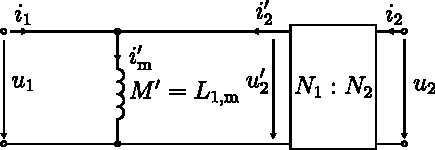
\includegraphics{fig/ex03/ex_transformer_T_ECD_core_losses_no_load.pdf}
    \caption{Equivalent circuit diagram without leakage flux and neglected winding and iron losses.}
    \label{fig:ex_transformer_T_ECD_core_losses_no_load}
  \end{solutionfigure}


  Therefore, the relationship between the voltage and flux linkage is given with:
  \begin{equation}
    u_{\mathrm{1}}(t) = -\frac{\mathrm{d}}{\mathrm{d}t} \psi(t),
  \end{equation}
  which is rearranged into the following form:
  \begin{equation}
    \psi = - \int u_{\mathrm{1}}(t) \mathrm{d}t
    = - \int \sqrt{2} U_{\mathrm{1}} \sin(\omega t) \mathrm{d}t.
  \end{equation}

  Due to the steady state, the integral is indefinite. This results in:
  \begin{equation}
    \psi = \frac{\sqrt{2}U_{\mathrm{1}}}{\omega} \cos(\omega t).
  \end{equation}

  This is simplified in the case of the maximum value of the flux linkage to:
  \begin{equation}
    \hat{\psi} = \frac{\sqrt{2}U_{\mathrm{1}}}{\omega}.
  \end{equation}

  The relationship between the flux linkage, the number of winding turns and flux is given with:
  \begin{equation}
    \psi = N_{\mathrm{1}} \phi_{\mathrm{1}}.
  \end{equation}


  Hence, the number of turns is calculated with:
  \begin{equation}
    N_{\mathrm{1}} = \frac{\hat{\psi}}{\phi}
    = \frac{\frac{\sqrt{2}U_{\mathrm{1}}}{\omega}}{\hat{B} S_{\mathrm{Fe}}}
    =\frac{\frac{\sqrt{2} \cdot \SI{230}{V}}{2\pi \cdot \SI{50}{\hertz}}}{\SI{0.8}{T} \cdot \SI{6\cdot 10^{-4}}{m}}
    = 2157.
    \label{eq:eq1}
  \end{equation}


  The turn ratio of the transformer is defined as follows
  \begin{equation}
    \ddot{u} = \frac{U_{\mathrm{1}}}{U_{\mathrm{2}}}
    = \frac{\SI{230}{\volt}}{\SI{48}{\volt}}
    = 4.79,
  \end{equation}
  hence, the winding turns for the secondary winding are calculated by:
  \begin{equation}
    N_{\mathrm{2}} = \frac{N_{\mathrm{1}}}{\ddot{u}}
    = \frac{2157}{4.79}
    = 451.
  \end{equation}

\end{solutionblock}


%%%%%%%%%%%%%%%%%%%%%%%%%%%%%%%%%%%%%%%%%%%%%%%%%%%%%%%%%%%%%
\subtask{Which magnetization current $I_{\mathrm{m}}'$ consumed the transformer in the no-load operating mode? Assume that the iron losses are neglected.}

\begin{solutionblock}
  
  At no-load operation, the current through the secondary winding is assumed to zero ($i_{\mathrm{2}} = \SI{0}{\ampere}$).
  
  Therefore, the electromotive force simplifies to:
  \begin{equation}
    \theta = H_{\mathrm{Fe}} l_{\mathrm{Fe}}
    = N_{\mathrm{1}} i_{\mathrm{1}}.
  \end{equation}

  Due to the no-load operation, the current through the primary winding is equal to the magnetization current. In addition, the maximum flux density $\hat{B}$ leads to the calculation of the peak magnetization current as:
  \begin{equation}
    \hat{i}_{\mathrm{1}} = \hat{i}_{\mathrm{m,1}}'
    = \frac{\hat{H}_{\mathrm{Fe}} l_{\mathrm{Fe}}}{N_{\mathrm{1}}}
    = \frac{\SI{2}{\ampere \per \centi \metre} \cdot \SI{30}{\centi \metre}}{2157}
    = \SI{27.8}{\milli \ampere}.
  \end{equation}


  The magnetic flux density $B$ shows a linear behavior in the area between 0 T and 0.8 T. Therefore, the magnetization current is not distorted due to the magnetization and has a sinusoidal characteristic.
  Hence, the current is calculated as follows:
  \begin{equation}
    I_{\mathrm{m}}' = \frac{\hat{i}_{\mathrm{m,1}}'}{\sqrt{2}}
    = \frac{\SI{27.8}{\milli\ampere}}{\sqrt{2}}
    = \SI{19.7}{\milli \ampere}.
  \end{equation}

  

\end{solutionblock}


%%%%%%%%%%%%%%%%%%%%%%%%%%%%%%%%%%%%%%%%%%%%%%%%%%%%%%%%%%%%%
\subtask{Calculate the factor between the peak magnetization current $\hat{i}_{\mathrm{m,2}}'$, when the applied voltage is risen from $U_{\mathrm{1}}$ = 230 V to $U_{\mathrm{1}}$ = 400 V.}

\begin{solutionblock}
  With the rearranged equation \eqref{eq:eq1}, the maximum flux density is calculated by:
  \begin{equation}
    \hat{B} = \frac{\sqrt{2} U_{\mathrm{1}}}{\omega S_{\mathrm{Fe}} N_{\mathrm{1}}}
    = \frac{\sqrt{2} \cdot \SI{400}{\volt}}{2\pi \cdot \SI{50}{\hertz} \cdot \SI{6 \cdot 10^{-4}}{\metre} \cdot 2157}
    = \SI{1.39}{\tesla}.
  \end{equation}

  The maximum flux density is used to determine the maximum field strength $\hat{H} = \SI{16}{\ampere \per \centi \metre}$. Hence, the peak magnetization current results in:
  \begin{equation}
    \hat{i}_{\mathrm{m,2}}' = \frac{\hat{H}_{\mathrm{Fe}} l_{\mathrm{Fe}}}{N_{\mathrm{1}}}
    = \frac{\SI{16}{\ampere \per \centi \metre} \cdot \SI{30}{\centi \metre}}{2157}
    = \SI{222.5}{\milli\ampere}.
  \end{equation}

  Hence, the factor is calculated as:
  \begin{equation}
    \frac{\hat{i}_{\mathrm{m,2}}}{\hat{i}_{\mathrm{m,1}}} = \frac{\SI{222.5}{\milli\ampere}}{\SI{27.8}{\milli\ampere}}
    = 8.
  \end{equation}
\end{solutionblock}



%%%%%%%%%%%%%%%%%%%%%%%%%%%%%%%%%%%%%%%%%%%%%%%%%%%%%%%%%%%%%
%% Task 4 %%
%%%%%%%%%%%%%%%%%%%%%%%%%%%%%%%%%%%%%%%%%%%%%%%%%%%%%%%%%%%%%

\task{Parameter identification via no-load test}
Given is a 50 Hz, 6 MVA single-phase transformer with $U_{\mathrm{1}}$ = 5 kV and $U_{\mathrm{2}}$ = 100 kV.
The effective area of the core is $S_{\mathrm{Fe}}$ = 0.187 $\mathrm{m}^2$ and a maximum flux density of $\hat{B}$ = 1.5 T. During the no-load operation, the primary voltage is $U_{\mathrm{1,o}}$ = 5 kV with a no-load electrical power $P_{\mathrm{o}}$ = 8.8 kW and the no-load current $I_{\mathrm{o}}$ = 2.6 A.



%%%%%%%%%%%%%%%%%%%%%%%%%%%%%%%%%%%%%%%%%%%%%%%%%%%%%%%%%%%%%
\subtask{Calculate the nominal currents and the transformer ratio.}

\begin{solutionblock}
  The transformer ratio is given as:
  \begin{equation}
    \ddot{u} = \frac{U_{\mathrm{1}}}{U_{\mathrm{2}}}
    = \frac{\SI{5}{\kilo \volt}}{\SI{100}{\kilo \volt}}
    = 0.05.
  \end{equation}

  With the apparent power $S$ of the transformer, the primary and secondary currents are calculated by:
  \begin{align}
    \begin{split}
      I_{\mathrm{1}} &= \frac{S}{U_{\mathrm{1}}}
      = \frac{\SI{6}{\mega \volt \ampere}}{\SI{5}{\kilo \volt}}
      = \SI{1200}{\ampere}, \\
      I_{\mathrm{2}} &= \frac{S}{U_{\mathrm{2}}}
      = \frac{\SI{6}{\mega \volt \ampere}}{\SI{100}{\kilo \volt}}
      = \SI{60}{\ampere}. \\
    \end{split}
  \end{align}

\end{solutionblock}



%%%%%%%%%%%%%%%%%%%%%%%%%%%%%%%%%%%%%%%%%%%%%%%%%%%%%%%%%%%%%
\subtask{Calculate the number of winding turns $N_{\mathrm{1}}$ for the primary and $N_{\mathrm{2}}$ for the secondary side.}

\begin{solutionblock}
  
  The number of winding turns for the primary side is calculated with:
  \begin{equation}
    N_{\mathrm{1}} = \frac{\hat{\psi}}{\phi}
    = \frac{\frac{\sqrt{2}U_{\mathrm{1}}}{\omega}}{\hat{B} S_{\mathrm{Fe}}}
    = \frac{\frac{\sqrt{2} \cdot \SI{5}{\kilo\volt}}{2\pi \cdot \SI{50}{\hertz}}}{\SI{1.5}{\tesla} \cdot \SI{0.187}{\metre^2}}
    = 81.
    \end{equation}

    The number of winding turns for the secondary side is calculated with the transformer ratio as follows:
    \begin{equation}
      N_{\mathrm{2}} = \frac{N_{\mathrm{1}}}{\ddot{u}}
      = \frac{81}{0.05}
      = 1620.
    \end{equation}
\end{solutionblock}

%%%%%%%%%%%%%%%%%%%%%%%%%%%%%%%%%%%%%%%%%%%%%%%%%%%%%%%%%%%%%
\subtask{Determine the iron losses and the apparent power $S_{\mathrm{o}}$ for no-load operation. Give the values for the magnetization current $I_{\mathrm{m}}'$, the iron loss current $I_{\mathrm{c}}$ and the mutual inductance $M'$. Assume for the calculation that $R_{\mathrm{1}} << R_{\mathrm{c}}$ and $L_{\mathrm{1,\sigma}} << M'$. In addition, draw the equivalent circuit diagram with the given assumptions.}


\begin{solutionblock}

  The equivalent circuit diagram for the no-load operation with the iron loss resistance $R_{\mathrm{c}}$ is shown in Fig.~\ref{fig:ex_transformer_open_circuit_test}.
  \begin{solutionfigure}
    \centering
    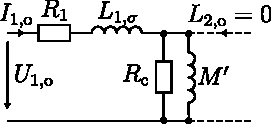
\includegraphics{fig/ex03/ex_Transformer_open_circuit_test.pdf}
    \captionsetup{labelfont={color=blue},textfont={color=blue}}
    \caption{Equivalent circuit diagram for the no-load test with the iron loss resistor $R_{\mathrm{c}}$.}
    \label{fig:ex_transformer_open_circuit_test}
  \end{solutionfigure}
  
  
  The no-load apparent power is calculated by
  \begin{equation}
    S_{\mathrm{o}} = U_{\mathrm{o}} I_{\mathrm{o}}
    = \SI{5}{\kilo\volt} \cdot \SI{2.6}{\ampere}
    = \SI{13}{\kilo\volt\ampere},
  \end{equation}
  with the no-load voltage $U_{\mathrm{o}}$ and the no-load current $I_{\mathrm{o}}$.

  The equivalent iron loss resistance is determine as follows
  \begin{equation}
    R_{\mathrm{c}} = \frac{U_{\mathrm{1,o}}^2}{P_{\mathrm{1,o}}}
    = \frac{\left(\SI{5}{\kilo\volt} \right)^2}{\SI{8.8}{\kilo\watt}}
    = \SI{2841}{\Omega},
  \end{equation}
  and, therefore, the corresponding current is calculated with:
  \begin{equation}
    I_{\mathrm{c}} = \sqrt{\frac{P_{\mathrm{1,o}}}{R_{\mathrm{c}}}}
    = \sqrt{\frac{\SI{8.8}{\kilo\watt}}{\SI{2841}{\Omega}}}
    = \SI{1.76}{\ampere}.
  \end{equation}

  The power factor is determined as
  \begin{equation}
    \cos \varphi_{\mathrm{o}} = \frac{P}{S}
    = \frac{\SI{8.8}{\kilo\watt}}{\SI{13}{\kilo\volt\ampere}}
    = 0.68,
  \end{equation}
  and the corresponding angle is $\varphi_{\mathrm{o}} = \SI{47.16}{\degree}$.

  The following equation is used to calculate the mutual inductance
  \begin{equation}
    \omega_{\mathrm{el}} M' \approx \frac{U_{\mathrm{1,o}}}{I_{\mathrm{1,o}} \sin(\varphi_{\mathrm{o}})},
  \end{equation}
  which is rearranged to:
  \begin{equation}
    M' = \frac{U_{\mathrm{1,o}}}{I_{\mathrm{1,o}} \sin(\varphi_{\mathrm{o}}) \omega_{\mathrm{el}}}
    = \frac{\SI{5}{\kilo\volt}}{\SI{2.6}{\ampere}\cdot \sin(\SI{47.16}{\degree})\cdot 2\pi \cdot \SI{50}{\hertz}}
    = \SI{8.35}{\henry}.
  \end{equation}

  With the geometric addition the magnetization currents is calculated with:
  \begin{equation}
    I_{\mathrm{m}}' = \sqrt{I_{\mathrm{1,o}}^2 - I_{\mathrm{c}}^2}
    = \sqrt{\left(\SI{2.6}{\ampere} \right)^2 - \left(\SI{1.76}{\ampere}\right)^2}
    = \SI{1.91}{\ampere}.
  \end{equation}

\end{solutionblock}







%%%%%%%%%%%%%%%%%%%%%%%%%%%%%%%%%%%%%%%%%%%%%%%%%%%%%%%%%%%%%
%% Task 5 %%
%%%%%%%%%%%%%%%%%%%%%%%%%%%%%%%%%%%%%%%%%%%%%%%%%%%%%%%%%%%%%

\task{Inrush current}
Given is a single-phase transformer in no-load operation (i.e., open circuit secondary side) which initial primary current is zero. A the time point $t$ = 0, the voltage $u_{\mathrm{n}}(t) = \hat{u}_{\mathrm{n}} \sin (\omega t + \alpha)$ is applied.
Remanence and iron losses are neglected.
The self-inductance $L_{\mathrm{1}}$, resistance $R_{\mathrm{1}}$ and the number of winding turns $N_{\mathrm{1}}$ are given.

%%%%%%%%%%%%%%%%%%%%%%%%%%%%%%%%%%%%%%%%%%%%%%%%%%%%%%%%%%%%%
\subtask{Calculate the inrush current trajectory $i_{\mathrm{1}}(t)$ and the trajectory of the flux $\phi (t)$.}

\begin{solutionblock}
  
  The dynamic equation of the transformer current is given as follows:
  \begin{equation}
    \frac{\mathrm{d}}{\mathrm{d}t}\bm{i}(t) = \begin{bmatrix} -\frac{R_1}{\sigma L_1} & \frac{R_2 M}{\sigma L_1 L_2} \\ \frac{R_1 M}{\sigma L_1 L_2} & -\frac{R_2}{\sigma L_2} \end{bmatrix} \bm{i}(t) + \begin{bmatrix} \frac{1}{\sigma L_1} & -\frac{M}{\sigma L_1 L_2} \\ -\frac{M}{\sigma L_1 L_2} & \frac{1}{\sigma L_2} \end{bmatrix} \bm{u}(t).
  \end{equation}

  Due to the no-load operation ($i_{\mathrm{2}} = \SI{0}{\ampere}$) and the neglected leakage flux, the equation simplifies to:
  \begin{equation}
    \frac{\mathrm{d}}{\mathrm{d}t} i_{\mathrm{1}}(t) = -\frac{R_{\mathrm{1}}}{L_{\mathrm{1}}}i_{\mathrm{1}}(t) -\frac{1}{L_{\mathrm{1}}} u_{\mathrm{1}}(t).
  \end{equation}

  The equation from above is rearranged to solve the ordinary differential equation. Therefore, the homogeneous part is on the left side and the perturbation part on the right side as given below
  \begin{equation}
    \frac{\mathrm{d}}{\mathrm{d}t} i_{\mathrm{1}}(t) + \frac{1}{\tau} i_{\mathrm{1}}(t) = \frac{1}{L_{\mathrm{1}}} u_{\mathrm{1}}(t),
    \label{eq:ode}
  \end{equation}
  with $\tau = \frac{L_{\mathrm{1}}}{R_{\mathrm{1}}}$.
  
  First, the homogeneous part is separated, which results in:
  \begin{equation}
    \frac{\mathrm{d}}{\mathrm{d}t} i_{\mathrm{1}}(t) + \frac{1}{\tau} i_{\mathrm{1}}(t) = 0.
  \end{equation}

  This homogeneous part is solved with the exponential approach, which is given with
  \begin{equation}
    i_{\mathrm{1}}(t) = C e^{-\frac{t}{\tau}},
    \label{eq:ode_approach_hom}
  \end{equation}
  and the first derivative
  \begin{equation}
    \frac{\mathrm{d}}{\mathrm{d}t}i_{\mathrm{1}}(t) = -\frac{C}{\tau} e^{-\frac{t}{\tau}},
    \label{eq:ode_approach_hom_derivative}
  \end{equation}
  with an integration constant $C$.

  Using \eqref{eq:ode_approach_hom} and \eqref{eq:ode_approach_hom_derivative} results in
  \begin{equation}
    \frac{R_{\mathrm{1}}}{L_{\mathrm{1}}} C e^{-\frac{t}{\tau}} - \frac{C}{\tau} e^{-\frac{t}{\tau}} = 0,
  \end{equation}
  which is rearranged as follows:
  \begin{equation}
    C e^{-\frac{t}{\tau}} \left(\frac{R_{\mathrm{1}}}{L_{\mathrm{1}}}-\frac{t}{\tau} \right)=0.
  \end{equation}


  Therefore, the homogeneous solution is given as:
  \begin{equation}
    i_{\mathrm{1,h}}(t) = C e^{-\frac{t}{\tau}}.
  \end{equation}
  

  In the second step, the perturbation solution is determined. Therefore, the comparison of coefficients ansatz is used.
  The voltage is given in the task with
  \begin{equation}
    u_{\mathrm{n}} = \hat{u}_{\mathrm{n}} \sin(\omega t + \alpha),
  \end{equation}
  which leads to:
  \begin{equation}
    \sin(\omega t + \alpha) = \cos(\omega t) \sin(\alpha) + \sin(\omega t) \cos(\alpha).
    \label{eq:ode_perturbation}
  \end{equation}

  The expression in \eqref{eq:ode_perturbation} is separated in two parts which are later combined again (superposition principle of linear systems). The approach for the first case is given by:
  \begin{equation}
    \frac{\mathrm{d}}{\mathrm{d}t}i(t) + \frac{1}{\tau}i(t) = k \sin(\alpha) \cos(\omega t),
  \end{equation}
  with a new parameter $k = \frac{\hat{u}}{L_{\mathrm{1}}}$, derived from \eqref{eq:ode}.

  The general approach is given with
  \begin{equation}
    i_{\mathrm{1,s}}(t) = a \cos(\omega t) + b \sin(\omega t),
    \label{eq:ode_approach_per}
  \end{equation}
  with the two parameter $a$ and $b$. The first derivative is determined as:
  \begin{equation}
    \frac{\mathrm{d}}{\mathrm{d}t} i_{\mathrm{1,s}}(t) = - a \omega \sin(\omega t) + b \omega \cos(\omega t).
    \label{eq:ode_approach_per_derivative}
  \end{equation}

  With \eqref{eq:ode_approach_per} and \eqref{eq:ode_approach_per_derivative} in \eqref{eq:ode} the equation is determined:
  \begin{equation}
    - a \omega \sin(\omega t) + b \omega \cos(\omega t) + \frac{1}{\tau} \left[a \cos(\omega t) + b \sin(\omega t)  \right]
    = k \sin(\alpha) \cos(\omega t).
  \end{equation}

  The following equation is obtained by reshaping
  \begin{equation}
    \sin(\omega t) \left[-a \omega + \frac{1}{\tau} b \right] + \cos(\omega t) \left[b\omega + \frac{1}{\tau} a - k \sin(\omega t) \right] = 0,
  \end{equation}
  and by dividing through $\cos(\omega t)$ results in:
  \begin{equation}
    \tan(\omega t) \left[-a \omega + \frac{1}{\tau} b \right] + \left[b \omega + \frac{1}{\tau}a - k \sin(\omega t) \right] = 0.
  \end{equation}

  To fulfill the equation, the expressions between the large brackets must be zero. 
  The first expression is given with:
  \begin{align}
    \begin{split}
      -a\omega + &\frac{1}{\tau}b = 0, \\
      b &= a \omega \tau.
      \label{eq:ode_b}
    \end{split}
  \end{align}

  The second expression is defined with:
  \begin{equation}
    b \omega + \frac{1}{\tau} a - k \sin(\alpha) = 0.
  \end{equation}

  With $b$ from \eqref{eq:ode_b} results in
  \begin{align}
    \begin{split}
      a \omega^2 \tau + \frac{1}{\tau} a - k \sin(\alpha) = 0, \\
      a \left[\omega^2 \tau + \frac{1}{\tau} \right] = k \sin(\alpha),
    \end{split}
  \end{align}

  which is reshaped to:
  \begin{equation}
    a = \frac{k \sin(\alpha)}{\omega^2 \tau + \frac{1}{\tau}}.
  \end{equation}

  Therefore, with the two calculated coefficients, the solution for the first approach is: 
  \begin{equation}
    i_{\mathrm{1,s}}(t) = \frac{k \sin(\alpha)}{\omega^2 \tau + \frac{1}{\tau}} \left[\cos(\omega t) + \omega \tau \sin(\omega t) \right].
  \end{equation}


  The second case is given with $\frac{\mathrm{d}}{\mathrm{d}t}i(t) + \frac{1}{\tau}i(t) = k \cos(\alpha) \sin(\omega t)$.To do this, the steps already carried out in the first approach are repeated.
  The starting point is given as
  \begin{equation}
    i_{\mathrm{2,s}}(t) = a \cos(\omega t) + b \sin(\omega t),
  \end{equation}
  and, therefore, the first derivative:
  \begin{equation}
    \frac{\mathrm{d}}{\mathrm{d}t} i_{\mathrm{2,s}}(t) = - a \omega \sin(\omega t) + b \omega \cos(\omega t).
  \end{equation}

  The comparison of coefficients and reshaping leads to:
  \begin{align}
    \begin{split}
    -a \omega \sin(\omega t) + b \omega \cos(\omega t) = \frac{1}{\tau} \left[a \cos(\omega t) + b\sin(\omega t) \right] &= k \sin(\omega t), \\
    \sin(\omega t) \left[-a \omega + \frac{1}{\tau}b - k\cos(\alpha)\right] + \cos(\omega t) \left[b \omega + \frac{1}{\tau}a \right] &= 0.
    \end{split}
  \end{align}

  To fulfill the equation, the expressions between the large brackets must be zero. 
  The first expression is given with:
  \begin{align}
    \begin{split}
      b \omega + &\frac{1}{\tau}a =0, \\
      a &= \omega b \tau.
      \label{eq:ode_parameter_a}
    \end{split}
  \end{align}

  The second expression is defined with:
  \begin{align}
    \begin{split}
      -a \omega + &\frac{1}{\tau}b - k\cos(\alpha) = 0, \\
      \omega^2 b \tau + &\frac{1}{\tau}b - k \cos(\alpha) = 0, \\
      b &= \frac{k\cos(\alpha)}{\omega^2\tau+\frac{1}{\tau}}.
    \end{split}
  \end{align}

  This result is used to solve parameter $a$ from \eqref{eq:ode_parameter_a} as follows:
  \begin{equation}
    a = -\omega b \tau = -\frac{\omega \tau k \cos(\alpha)}{\omega^2\tau + \frac{1}{\tau}}.
  \end{equation}

  Therefore, the solution for the second case of the perturbation part is defined as
  \begin{equation}
    i_{\mathrm{s,2}}(t) = \frac{k\cos(\alpha)}{\omega^2 \tau + \frac{1}{\tau}} \left[-\omega \tau \cos(\omega t) + \sin(\omega t) \right],
    \end{equation}

 and, this leads to the solution of the perturbation part by:
  \begin{equation}
    i_{\mathrm{1,s}}(t) = \frac{k}{\omega^2 \tau + \frac{1}{\tau}}
    \left[
      \sin(\alpha)\left[\cos(\omega t) + \omega \tau \sin(\omega t) \right]
      + \cos(\alpha) \left[-\omega \tau \cos(\omega t) + \sin(\omega t) \right]
    \right].
  \end{equation}

  The total solution is given with:
  \begin{equation}
    i_{\mathrm{1}}(t) = i_{\mathrm{1,h}}(t) + i_{\mathrm{1,s}}(t).
  \end{equation}


  Next, the integration constant $C$ from the homogeneous solution is determined. To perform this, the initial conditions are used, which are defined in the task description. Therefore, the current is defined as:
  \begin{equation}
    i_{\mathrm{1}}(0) = 0.
    \label{eq:ode_initialCondition}
  \end{equation}
  
  The second initial condition is the results of applying \eqref{eq:ode_initialCondition} to the differential equation, that is:
  \begin{equation}
    \frac{\mathrm{d}}{\mathrm{d}t}i_{\mathrm{1}}(0) = \frac{1}{L_{\mathrm{1}}}u(0) = \frac{1}{L_{\mathrm{1}}} \hat{u}\sin(\alpha).
  \end{equation}

  Apply the initial conditions to the total solution results in
  \begin{equation}
    i(0) = C + \frac{k}{\omega^2 \tau + \frac{1}{\tau}}
    \left[\sin(\alpha) - \omega \tau \cos(\alpha) \right] = 0,
  \end{equation}
  which is rearranged to:
  \begin{equation}
    C = \frac{k}{\omega^2\tau + \frac{1}{\tau}} \left[-\sin(\alpha) + \omega \tau \cos(\alpha) \right].
  \end{equation}

  Therefore, the total solution is given with:
  \begin{align}
    \begin{split}
      i_{\mathrm{1}}(t) &=\frac{k}{\omega^2\tau + \frac{1}{\tau}} \left[-\sin(\alpha) + \omega \tau \cos(\alpha) \right] e^{-\frac{t}{\tau}} \\
      &+\frac{k}{\omega^2 \tau + \frac{1}{\tau}}
      \left[
        \sin(\alpha)\left[\cos(\omega t) + \omega \tau \sin(\omega t) \right]
        + \cos(\alpha) \left[-\omega \tau \cos(\omega t) + \sin(\omega t) \right]
      \right].
      \label{eq:ode_solution}
  \end{split}
  \end{align}

  The trajectory of the flux is defined as
  \begin{equation}
    \phi(t) = L_{\mathrm{1}} i(t),
  \end{equation}
  and, therefore, directly given with the current trajectory.
\end{solutionblock}



%%%%%%%%%%%%%%%%%%%%%%%%%%%%%%%%%%%%%%%%%%%%%%%%%%%%%%%%%%%%%
\subtask{Assume that $R_{\mathrm{1}} << \omega L_{\mathrm{1}}$.
Discuss the result for $i_{\mathrm{1}}(t)$, when the voltage is applied at zero crossing with an angle $\alpha$ = 0 and for an angle of $\alpha = \frac{\pi}{2}$.}

\begin{solutionblock}

  First, the trajectory for $\alpha$ = 0 is determined. Therefore, \eqref{eq:ode_solution} results in:
  \begin{equation}
    i_{\mathrm{1}}(t) = \frac{k}{\omega^2\tau+\frac{1}{\tau}} \left[\omega \tau e^{-\frac{t}{\tau}} - \omega \tau \cos(\omega t) + \sin(\omega t) \right].
  \end{equation}

  With the assumptions given in the task, $R_{\mathrm{1}} << L_{\mathrm{1}} \omega$
  results into $\omega \tau >> 1$.

  Hence, the equation simplifies to
  \begin{align}
    \begin{split}
      i_{\mathrm{1}}(t) &= \frac{k}{\omega^2\tau + \frac{1}{\tau}} \omega t \left[e^{-\frac{t}{\tau}} - \cos(\omega t) \right], \\
      &= \frac{\hat{u}}{L_{\mathrm{1}}} \frac{1}{\omega} \left[e^{-\frac{t}{\tau}} - \cos(\omega t) \right],
    \end{split}
  \end{align}
  which is used to calculate the current trajectory. 
  As it can be seen, the equation contains an exponential part. To determine the steady-state current trajectory, the equation is reshaped into:
  \begin{align}
    \begin{split}
    i_{\mathrm{1}}(t) = \frac{\hat{u}}{L_{\mathrm{1}}\omega}e^{-\frac{t}{\tau}}-\frac{\hat{u}}{L_{\mathrm{1}}\omega}\cos(\omega t), \\
    = \frac{\hat{u}}{L_{\mathrm{1}}\omega}e^{-\frac{t}{\tau}} + \frac{\hat{u}}{L_{\mathrm{1}}} \int \sin(\omega t) \mathrm{d}t.
    \end{split}
  \end{align}

  With the input voltage $u(t) = \hat{u}\sin(\omega t + \alpha)$, the equation simplifies to:
  \begin{equation}
    i_{\mathrm{1}}(t) = \frac{\hat{U}}{L_{\mathrm{1}}\omega}e^{-\frac{t}{\tau}} + \frac{1}{L_{\mathrm{1}}} \int u(t) \mathrm{d}t.
  \end{equation}

  Assumed, that in the steady state $\tau \rightarrow \infty$, only the second part of the equation remains. Therefore, the current trajectory is given with:
  \begin{equation}
    i_{\mathrm{1}}(t) = \frac{1}{L_{\mathrm{1}}} \int u(t) \mathrm{d}t.
  \end{equation}

  Next, the trajectory for $\alpha = \frac{\pi}{2}$ is determined. Therefore, the equation \eqref{eq:ode_solution} is solved as follows:
  \begin{align}
    \begin{split}
      i_{\mathrm{1}}(t) &= \frac{k}{\omega^2\tau + \frac{1}{\tau}}
      \left[\cos(\omega t) + \omega \tau \sin(\omega t) \right], \\
      &= \frac{k}{\omega^2\tau + \frac{1}{\tau}} \left[\omega \tau \sin(\omega t) \right], \\
      &= \frac{1}{L_{\mathrm{1}}} \hat{U} \frac{1}{\omega} \sin(\omega t), \\
      &= \frac{\hat{U}}{L_{\mathrm{1}}\omega} \sin(\omega t).
    \end{split}
  \end{align}


  In Fig.~\ref{fig:current_transformer} the two calculated current trajectories are visualized. They result from the applied voltage with the additional angle $\alpha$.
  In this example is the peak current value during the transient process approximately double than in the steady state, which can trigger the overcurrent protection. Therefore, the magnetization current should be kept low and the overcurrent protection must be able to handle the inrush current.
  \begin{solutionfigure}
    \centering
    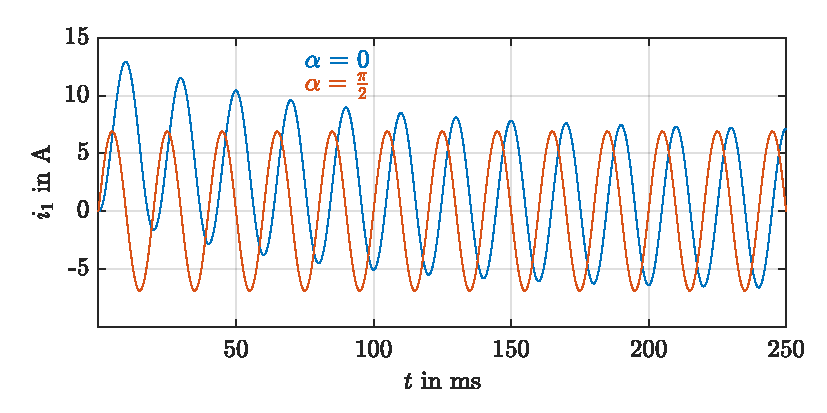
\includegraphics{fig/ex03/current_transformer.pdf}
    \caption{Current of the transformer, when the voltage is applied at two different angles for $\alpha$.}
    \label{fig:current_transformer}
  \end{solutionfigure}
  

\end{solutionblock}

\end{document}